\documentclass[a4paper]{report}

%====================== PACKAGES ======================
\usepackage[top=2cm, bottom=2cm, left=2cm, right=2cm]{geometry}
\usepackage[utf8]{inputenc}
\usepackage[T1]{fontenc}
\usepackage{amsmath,amsfonts,amssymb}

\usepackage[french]{babel}
%pour gérer les positionnement d'images
\usepackage{float}
\usepackage{array}
\usepackage{enumitem}
\usepackage{multirow}
\usepackage{mathpazo}
\usepackage{multicol}
\usepackage{nicefrac}
\usepackage{graphicx, epsfig}
\usepackage[colorinlistoftodos]{todonotes}
\usepackage{url}
%pour les informations sur un document compilé en PDF et les liens externes / internes
\usepackage{hyperref}
%pour la mise en page des tableaux
\usepackage{array}
\usepackage{tabularx}
%pour utiliser \floatbarrier
%\usepackage{placeins}
%\usepackage{floatrow}
%espacement entre les lignes
\usepackage{setspace}
%modifier la mise en page de l'abstract
\usepackage{abstract}
%police et mise en page (marges) du document
\usepackage[T1]{fontenc}
\usepackage[top=2cm, bottom=2cm, left=2cm, right=2cm]{geometry}
%Pour les galerie d'images
\usepackage{subfig}
\usepackage{etoolbox}

\makeatletter
% First, modify the \@endpart macro.
\def\@endpart{} 

% Next, copy the \chapter macro to \nonewpagechapter, and ...
% ... suppress page-breaking instructions in the modified macro
\let\nonewpagechapter\chapter 
\patchcmd\nonewpagechapter{\if@openright\cleardoublepage\else\clearpage\fi}{}{}{}

% Third, suppress vertical whitespace before "Part xx" material
\patchcmd{\part}{\null\vfil}{}{}{}

\makeatother


%----------------------------------------------------------------------------
%   APPENDICES
%----------------------------------------------------------------------------
\usepackage[toc,page]{appendix}
\renewcommand{\appendixpagename}{Annexes}
\renewcommand{\appendixtocname}{Annexes}


%====================== INFORMATION ET REGLES ======================

%rajouter les numérotation pour les \paragraphe et \subparagraphe
\setcounter{secnumdepth}{4}
\setcounter{tocdepth}{4}

\hypersetup{							% Information sur le document
pdfauthor = {BENELKATER Mohamed,
			BURBANO Paula,
			COMBARET Léo,
    		PREVOT Alexia,
    		RAKOTOVAO Jonathan},			% Auteurs
pdftitle = {Analyse numérique d’instruments à cordes},			% Titre du document
pdfsubject = {Mémoire de Projet},		% Sujet
pdfkeywords = {Tag1, Tag2, Tag3, ...},	% Mots-clefs
pdfstartview={FitH}}					% ajuste la page à la largueur de l'écran
%pdfcreator = {MikTeX},% Logiciel qui a crée le document
%pdfproducer = {}} % Société avec produit le logiciel

%======================== DEBUT DU DOCUMENT ========================

\begin{document}

%régler l'espacement entre les lignes
\newcommand{\HRule}{\rule{\linewidth}{0.5mm}}

%page de garde
\begin{titlepage}
\begin{center}

% Upper part of the page. The '~' is needed because only works if a paragraph has started.

\includegraphics[width=0.35\textwidth]{./Logo_Polytech_Sorbonne}~\\[1cm]

\textsc{\LARGE Polytech Sorbonne}\\[1.5cm]

\textsc{\Large }\\[0.5cm]

% Title
\HRule \\[0.4cm]

{\huge \bfseries Projet\\
Analyse numérique d’instruments à cordes \\[0.4cm] }

\HRule \\[1.5cm]

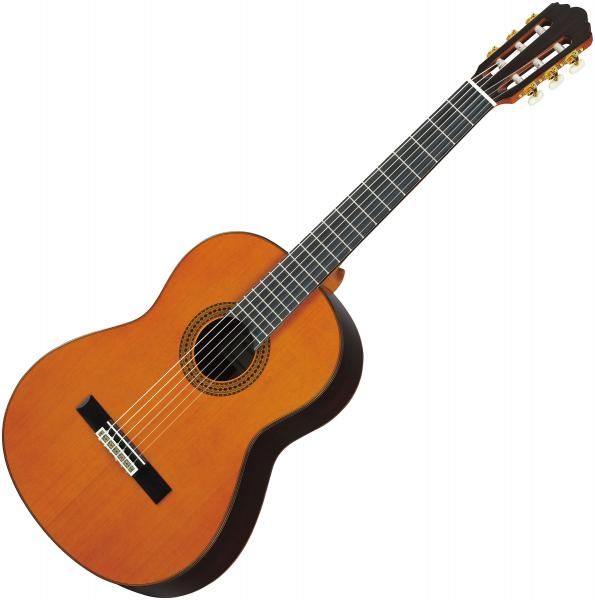
\includegraphics[width=0.35\textwidth]{./guitare}~\\[1cm]

% Author and supervisor
\begin{minipage}{0.4\textwidth}
\begin{flushleft} \large
BENELKATER \textsc{Mohamed}\\
BURBANO \textsc{Paula}\\
COMBARET \textsc{Léo}\\
FIDA CYRILLE \textsc{Rudio}\\
PREVOT \textsc{Alexia}\\
RAKOTOVAO \textsc{Jonathan}
\end{flushleft}
\end{minipage}
\begin{minipage}{0.4\textwidth}
\begin{flushright} \large
\emph{Encadrant:} \\
Yann \textsc{TEYTAUT}\\
\emph{MAIN3} \\
2020/2021
\end{flushright}
\end{minipage}

\vfill

% Bottom of the page
{\large \today}

\end{center}
\end{titlepage}


\tableofcontents
\thispagestyle{empty}
\setcounter{page}{0}
%ne pas numéroter le sommaire


%espacement entre les lignes d'un tableau
\renewcommand{\arraystretch}{1.5}

%====================== INCLUSION DES PARTIES ======================

~
\thispagestyle{empty}
%recommencer la numérotation des pages à "1"
\setcounter{page}{0}
\newpage
\makeatletter\@addtoreset{section}{part}\makeatother
\renewcommand{\thesection}{\arabic{section}}

\part{Présentation du projet}

\section{Mise en contexte}

Une onde est la propagation d'une perturbation qui se déplace à une certaine vitesse et possédant des propriétés physiques. Sans s'en rendre compte, nous avons à faire à ces ondes tous les jours lorsque nous regardons les ondulations d'une flaque d'eau produites par des gouttes d'eau, ou simplement dès lors qu'on ouvre les yeux et qu'on capte la lumière provenant des objets qui nous entourent. Ainsi, en savoir plus sur ces ondes et comprendre comment elles fonctionnent semble être un travail intéressant.

Lors de ce projet pluridisciplinaire, nous nous penchons sur l'étude d'ondes mécaniques se propageant sur le long d'une corde d'un instrument à cordes.


\section{Sujet}

Dans le cadre de ce projet, nous cherchons à appliquer des méthodes d'analyse numérique à un instrument à corde. En effet, nous pouvons nous demander comment modéliser numériquement une onde dans une corde de guitare. 

\section{Objectif : comparer des méthodes de résolution numérique de l'équation d'onde}

L'objectif premier est de se familiariser avec le domaine physique des ondes et de chercher comment modéliser l'onde se propageant le long d'instruments à cordes. Nous serons confrontés à une équation dite équation d'onde ou équation de D'Alembert. Il sera alors nécessaire de l'étudier, la comprendre et utiliser des méthodes d'analyse numérique afin d'approcher une solution à cette équation. Par ailleurs, il sera intéressant de comparer différentes méthodes d'analyse numérique en prenant en compte des critères de stabilité, rapidité, efficacité, etc.

\section{Idée de la démarche générale}

Pour cela, nous allons étudier et comprendre différentes méthodes d'analyse numérique basée sur la discrétisation puis les appliquer mathématiquement pour notre équation.
\newline
Les différentes méthodes sont les suivantes:
\begin{itemize}
    \item la méthode d'Euler explicite;
    \item la méthode d'Euler implicite;
    \item la méthode de Runge-Kutta.
\end{itemize}
Ensuite on les implémentera en code python et visualisera les résultats. Nous pourrons alors analyser la stabilité des modèles en faisant varier les paramètres (conditions initiales,pas de discrétisation).Enfin, nous confronterons les méthodes de discrétisation en comparant les résultats, les erreurs et nous ferons varier les conditions initiales.\\




\part{Étude de l'équation des ondes}

\section{Caractérisation du problème}

\subsection{Présentation de l'équation}

L'équation de D'Alembert (appelée aussi équation d'onde ou équation des ondes) est l'équation générale qui décrit la propagation d'une onde, qui peut être représentée par une grandeur scalaire ou vectorielle. 
Elle s'écrit : 

\begin{equation*}
\frac{\partial^2u}{\partial t^2} = c^{2}\frac{\partial^2u}{\partial x^2}
\end{equation*}
 
    avec $c$ la célérité d'onde \\
Pour la résoudre, nous avons besoin de la condition de Neumann :
\begin{equation*}
\frac{\partial u}{\partial t} (0,x) = f(x)
\end{equation*}
et de la condition de Dirichlet : $u(0,x) = g(x)$\\
où f et g sont des fonctions quelconques d'une seule variable.\\

Cette équation peut être résolue mathématiquement (solution dite exacte) pour des modèles simples tels que celui d'une corde que l'on étudiera. La solution exacte de l'équation d'onde est de la forme :
$u(t,x) = f(x-ct) + g(x+ct)$ avec $f$ et $g$ des fonctions quelconques d'une seule variable.  \\

Cependant, dans ce projet, on s'intéressera à appliquer des méthodes d'analyse numérique pour résoudre l'équation d'onde (solutions approchées).\\

Des ondes stationnaires sont créées sur la corde par le musicien. Comme dans le problème, la corde est fixée, il faut que la fonction $u(x,t)$ s'annule sur ses bornes.\\
On obtient alors les conditions initiales suivantes :\\
\begin{equation*}
\left \{
\begin{array}{rcl}
u(0,t)=0\\
u(L,t)=0\\
\end{array}
\right.
\end{equation*}\\


\section{Étude physique de la corde}

La vitesse de propagation de l'onde sur la corde dépend de la tension de celle-ci:

\begin{equation*}
c = \sqrt{\frac{\tau}{\rho}}
\end{equation*}

avec \\
\hspace*{2cm} $\tau$ qui représente la tension, \\
\hspace*{2cm} $\rho$ la masse par unité de longueur, ou densité linéique.\\

Plus une corde est tendue, plus la vitesse de propagation d’une onde y sera élevée.\

On prendra par la suite comme valeurs 0,5 m pour la longueur $l$ de cette corde et 5,8.10-3 kg.m-1 pour la densité linéique $\rho$.\

On pourra alors faire varier la tension de la corde et en observer les conséquences.




\part{Discrétisation et modélisation}

\section{Principe}

On  considère  une  équation  différentielle  ordinaire  (EDO) $u'(t)=f(t,u(t))$. Lorsqu'on ne  connaît pas de solution exacte à cette EDO, on essaye d'en avoir une bonne approximation par  des méthodes numériques.

Cette équation décrit comment varie une fonction, en un point donné (un instant ou un point de l'espace), connaissant la valeur de cette fonction mathématique, le problème à résoudre s'écrit:

\begin{equation*}
\left \{
\begin{array}{rcl}
u'(t)=f(t,u(t))\\
u(t=t_0) = u_0 \\
\end{array}
\right.
\end{equation*}

Nous  allons par  exemple  observer  $u$  sur un intervalle de  temps
régulier de pas $h$. Nous  allons  essayer  d'obtenir  une suite  d'approximations  $u_n$  de
$u(t_n)$.\\

Considérons le problème monodimensionnel de la vibration d'une corde de guitare. Le schéma de la vibration de guitare vérifie l'équation de D'Alembert :
\begin{equation*}
\frac{\partial^2u}{\partial t^2} = c^{2}\frac{\partial^2u}{\partial x^2}
\end{equation*}
où $c$ est la vitesse de l'onde.\\

Ici, il ne s'agit pas d'une EDO mais d'une EDP (Equation aux Dérivées Partielles). Nous allons donc utiliser la méthode des différences finies.\\

La première étape consiste à discrétiser l'espace et le temps en des nombres finis d'intervalles de dimension connue appelé pas de discrétisation, respectivement $\Delta x$ et $\Delta t$. C'est le maillage.

On remplace ensuite les dérivées apparaissant dans l'équation par des quotients aux différences obtenus à partir d'un développement de Taylor à un ordre fixé selon la précision recherchée. Il s'agit de la méthode des différences finies qui permet d'approcher les valeurs des dérivées.\\

\section{Méthodes d'Euler}

L'intervalle $[0,L]$ est discrétisé en $Nx+1$ noeuds de coordonnées $x_{i}$ ($i$ variant de $0$ à $N$) régulièrement espacés. Notons $\Delta x$ le pas d'espace. L'intervalle de temps $[0,T]$ est discrétisé quant à lui en Nt intervalles de pas constant $\Delta t$. Notons $u^{n}_{i}$ l'amplitude de la corde au noeud $x_{i} = i\Delta x$ et à l'instant $t = n\Delta t$.\\\\

\subsection{Schéma Explicite}

La méthode d'Euler explicite consiste à considérer que, d'un point $t^n_{i}$ au point $t^{n+1}_{i}$, la fonction évolue linéairement, avec une trajectoire qui est celle qu'on peut calculer au point $t_i$.\\
On peut alors approximer la fonction $(u(t_n,x_i)$ en  calculant $u^{n+1}_{i}$ connaissant $u^n_{i}$.\\


Le problème se résoud donc de la façon suivante:\\
$\rightarrow$ on connaît la fonction f, un point tn où on connaît $u^n_{i}$\\
$\rightarrow$ on peut donc calculer $u'(t)=f(t,u(t))$ \\
$\rightarrow$ on estime alors la valeur de u au point $t_{n+1} = t_n + \Delta t$ : $u_{n+1} \approx u_n + u'_n\Delta t$\\
$\rightarrow$ on peut alors itérer (résoudre pas à pas) pour passer au point suivant. Le problème est initialisé en partant de $t_0$ où on connaît $u_0$ (condition à la limite).\\


On obtient à partir de le méthode des différences finies les schémas centré d'ordre 2 pour les dérivées spatiale et temporelle : 
\begin{equation*}
(\frac{\partial^2u}{\partial t^2})^{n}_{i} = \frac{u^{n+1}_{i} - 2u^{n}_{i} + u^{n-1}_{i}}{\Delta t^2}
\end{equation*}
\vspace*{3 mm}
\begin{equation*}
(\frac{\partial^2u}{\partial x^2})^{n}_{i} = \frac{u^{n}_{i+1} - 2u^{n}_{i} + u^{n}_{i-1}}{\Delta x^2}
\end{equation*}
\vspace*{3 mm}
\begin{equation*}
\frac{u^{n+1}_{i} - 2u^{n}_{i} + u^{n-1}_{i}}{\Delta t^2} = c^2 \frac{u^{n}_{i+1} - 2u^{n}_{i} + u^{n}_{i-1}}{\Delta x^2}
\end{equation*}
\hspace*{0.6cm} On pose :
\begin{equation*}
\lambda = c \frac{\Delta t}{\Delta x}
\end{equation*}
\hspace*{0.6cm} ce qui donne
\begin{equation*}
u^{n+1}_{i} - 2u^{n}_{i} + u^{n-1}_{i} = \lambda ^2 (u^{n}_{i+1} - 2u^{n}_{i} + u^{n}_{i-1})
\end{equation*}
\vspace*{3 mm}
\begin{equation*}
\Leftrightarrow
\boxed{
u^{n+1}_{i} = \lambda ^2 u^{n}_{i+1} + (2 - 2\lambda ^2)u^{n}_{i} - u^{n-1}_{i} + \lambda ^2 u^{n}_{i-1}}
\end{equation*}

\vspace*{7 mm}

Posons U = 
\begin{math}
\begin{pmatrix}
u_{1}\\
u_{2}\\
\vdots \\
\vdots \\
u_{N-2}\\
u_{N-1}
\end{pmatrix}
, \hspace{3 mm} A = 
\begin{pmatrix}
(2-2\lambda ^2) & \lambda ^2 & 0 & \cdots & \cdots & 0\\
\lambda ^2 & (2-2\lambda ^2) & \lambda ^2 & 0 & \cdots & \vdots\\
0 & \ddots & \ddots & \ddots & \cdots & \vdots\\
\vdots & \vdots & \ddots & \ddots & \ddots & 0\\
\vdots & \vdots & 0 &\lambda ^2 & (2-2\lambda ^2) & \lambda ^2 \\
0 & \cdots & \cdots & 0 & \lambda ^2 & (2-2\lambda ^2)
\end{pmatrix}
et \hspace{3 mm} C = 
\begin{pmatrix}
u_{l0}\\
0\\
\vdots \\
\vdots \\
0\\
u_{lN}
\end{pmatrix}
\end{math}

\vspace*{7 mm}
alors\\

\begin{equation*}
U^{n+1}_i = A.U^{n}_i - U^{n-1}_i + C_i\\
\end{equation*}

On va donc résoudre cette équation en prenant des conditions initiales cohérentes. La corde de guitare est fixée à ses extrémités et admet un momentum initial lorsque t=0 (que l'on définira lors des expérimentations).

Conditions initiales: 
\begin{equation*}
\left \{
\begin{array}{rcl}
u^{n}_{0}& = & 0 \hspace*{4 mm} \forall n\\
u^{n}_{L}& = &0 \hspace*{4 mm} \forall n\\
\end{array}
\right.
\end{equation*}

Donc $C = 0$\\

Soit
\begin{equation*}
\boxed{
U^{n+1}_i = A.U^{n}_i - U^{n-1}_i}
\end{equation*}

On a donc la formule de récurrence cherchée pour approximer la suite $u^n_i$.
\newline
\newline
De plus, nous avons besoin de déterminer $u^1_i$ $\forall i$ pour utiliser notre schéma d'Euler. Ainsi, l'on utilise les conditions initiales du problème pour obtenir ces valeurs:
\begin{equation*}
\left \{
\begin{array}{rcl}
\frac{\partial u}{\partial t} (0,x) = f(x)\hspace*{4 mm}\\
 u(0,x) = g(x) \hspace*{4 mm} \\
\end{array}
\right.
\end{equation*}

On a donc par la méthode des différences finies:
\begin{equation*}
\frac{u^{n+1}_{i} - u^{n}_{i}}{\Delta t} = \frac{\partial u}{\partial t}
\end{equation*}
\begin{equation*}
\Leftrightarrow \frac{u^{1}_{i} - u^{0}_{i}}{\Delta t} = \frac{\partial u(x,0)}{\partial t}
\end{equation*}
\begin{equation*}
\Leftrightarrow \frac{\partial u(x,0)}{\partial t} = \frac{u^{1}_{i} - u^{0}_{i}}{\Delta t}
\end{equation*}
\begin{equation*}
\Leftrightarrow u^{1}_{i} = \Delta t \frac{\partial u(x,0)}{\partial t} + u^{0}_{i}
\end{equation*}\\
D'où:
\begin{equation*}
\left \{
\begin{array}{rcl}
u^0_i = u(x,0) \hspace*{4 mm} \forall n\\
u^1_i = \Delta t \frac{\partial u(x,0)}{\partial t} + u(x,0) \hspace*{4 mm} \forall n\\
\end{array}
\right.
\end{equation*}
\\
La description de l'algorithme utilisé est à retrouver en annexe 3.\\ Le code python est accessible via le lien github en annexe 4.

\subsection{Schéma Implicite}

On reprend ici les mêmes notations. La méthode d'Euler implicite consiste à chercher la valeur approchée à l'instant $t_{n+1}$ avec la relation suivante :
$u^{n+1}_i \approx u^n_i + u'^{n+1}_i\Delta t$\\

On va donc utiliser une approche pour discrétiser l'équation au noeud $x_{i}$ et à l'itération $n+1$:\\
\begin{equation*}
(\frac{\partial u}{\partial t})^{n+1}_{i} = c^2 (\frac{\partial^2u}{\partial t^2})^{n+1}_{i}
\end{equation*}
Nous utilisons un schéma arrière d'ordre 2 pour évaluer la dérivée seconde temporelle:
\begin{equation*}
(\frac{\partial^2u}{\partial t^2})^{n+1}_{i} = \frac{u^{n+1}_{i} - 2u^{n}_{i} + u^{n-1}_{i}}{\Delta t^2}
\end{equation*}
Ainsi qu'un schéma centré d'ordre 2 pour la dérivée seconde en espace:
\begin{equation*}
(\frac{\partial^2u}{\partial x^2})^{n+1}_{i} = \frac{u^{n+1}_{i+1} - 2u^{n+1}_{i} + u^{n+1}_{i-1}}{\Delta x^2}
\end{equation*}
On pose :
\begin{equation*}
\lambda = c \frac{\Delta t}{\Delta x}
\end{equation*}
Alors d'après l'équation de discrétisation:
\begin{equation*}
(\frac{\partial u}{\partial t})^{n+1}_{i} = c^2 (\frac{\partial^2u}{\partial t^2})^{n+1}_{i}
\end{equation*}
\begin{equation*}
\Leftrightarrow\frac{u^{n+1}_{i} - 2u^{n}_{i} + u^{n-1}_{i}}{\Delta t^2} = c^2 \frac{u^{n+1}_{i+1} - 2u^{n+1}_{i} + u^{n+1}_{i-1}}{\Delta x^2}
\end{equation*}
\begin{equation*}
\Leftrightarrow u^{n+1}_{i} - 2u^{n}_{i} + u^{n-1}_{i} = \lambda ^2 (u^{n+1}_{i+1} - 2u^{n+1}_{i} + u^{n+1}_{i-1})
\end{equation*}
\begin{equation*}
\Leftrightarrow u^{n+1}_{i} - 2u^{n}_{i} + u^{n-1}_{i} = \lambda ^2 (u^{n+1}_{i+1} - 2u^{n+1}_{i} + u^{n+1}_{i-1})
\end{equation*}
\begin{equation*}
\Leftrightarrow - 2u^{n}_{i} = \lambda ^2 (u^{n+1}_{i+1} - 2u^{n+1}_{i} + u^{n+1}_{i-1}) - (u^{n+1}_{i} + u^{n-1}_{i})
\end{equation*}
\begin{equation*}
\Leftrightarrow u^{n}_{i} = \frac{-\lambda ^2}{2} (u^{n+1}_{i+1} - 2u^{n+1}_{i} + u^{n+1}_{i-1}) + \frac{1}{2} (u^{n+1}_{i} + u^{n-1}_{i})
\end{equation*}
\begin{equation*}
\Leftrightarrow
\boxed{
u^{n}_{i} = \frac{-\lambda ^2}{2}u^{n+1}_{i+1} + (\lambda^2 + \frac{1}{2})u^{n+1}_{i} - \frac{\lambda ^2}{2}u^{n+1}_{i-1} + \frac{1}{2} u^{n-1}_{i}}
\end{equation*} \\\\
Ecriture de l'équation sous forme matricielle: \vspace{3 mm}\\

Posons U = 
\begin{math}
\begin{pmatrix}
u_{1}\\
u_{2}\\
\vdots \\
\vdots \\
u_{N-2}\\
u_{N-1}
\end{pmatrix}
, \hspace{3 mm} A = 
\begin{pmatrix}
(\lambda ^2 + \frac{1}{2}) & \frac{-\lambda ^2}{2} & 0 & \cdots & \cdots & 0\\
\frac{-\lambda ^2}{2} & (\lambda ^2 + \frac{1}{2}) & \frac{-\lambda ^2}{2} & 0 & \cdots & \vdots\\
0 & \ddots & \ddots & \ddots & \cdots & \vdots\\
\vdots & \vdots & \ddots & \ddots & \ddots & 0\\
\vdots & \vdots & 0 &\frac{-\lambda ^2}{2} & (\lambda ^2 + \frac{1}{2}) & \frac{-\lambda ^2}{2} \\
0 & \cdots & \cdots & 0 & \frac{-\lambda ^2}{2} & (\lambda ^2 + \frac{1}{2})
\end{pmatrix}
et \hspace{3 mm} C = 
\begin{pmatrix}
u_{g}\\
0 \\
\vdots \\
\vdots \\
0 \\
u_{d}
\end{pmatrix}
\end{math}\\\\
alors
\begin{equation*}
U^{n}_i = A.U^{n+1}_i - \frac{\lambda^2}{2}.C_i+\frac{1}{2}.U^{n-1}_i
\end{equation*}

On va donc résoudre cette équation en prenant des conditions initiales cohérentes.\\
La corde de guitare est fixée à ses extrémités donc les points lorsque $x = 0$ et $x = L$ gardent leur position initiale.\\
Conditions initiales sur $x$: 
\begin{equation*}
\left \{
\begin{array}{rcl}
u(0,t) = u_{g} = &0 \hspace*{4 mm} \forall n\\
u(L,t) = u_{d} = &0 \hspace*{4 mm} \forall n\\
\end{array}
\right.
\end{equation*}
Donc $C = 0$\\
Soit
\begin{equation*}
\boxed{
A.U^{n+1}_i = U^{n}_i - \frac{1}{2}.U^{n-1}_i\:
et\:
U^{n+1}_i = A^{-1}(U^{n}_i - \frac{1}{2}.U^{n-1}_i)}
\end{equation*}



D'autre part, la corde admet un momentum initial $\forall x$ à l'instant $t=0$. La position de la corde à $t = 0$ sera définie lors de l'expérimentation car il existe plusieurs modèles de momentum initial qui peuvent faire varier les résultats.\\

De la même manière que pour la méthode explicite, on obtient les conditions initiales :
\begin{equation*}
\left \{
\begin{array}{rcl}
u^0_i = u(x,0) \hspace*{4 mm} \forall n\\
u^1_i = \Delta t \frac{\partial u(x,0)}{\partial t} + u(x,0) \hspace*{4 mm} \forall n\\
\end{array}
\right.
\end{equation*}
\\
La description de l'algorithme utilisé est à retrouver en annexe 3.\\ Le code python est accessible via le lien github en annexe 4.

\section{Méthode de Runge-Kutta}

Les méthodes de Runge-Kutta sont des schémas numériques à un pas qui permettent de résoudre des équations différentielles ordinaires.
Elles sont appréciées pour leur précision grâce à des ordres plus élevés: 2 ou 4.\\

Dans le cas de l'équation d'onde, l'utilisation d'une méthode de Runge Kutta n'est pas évidente étant donné qu'il s'agit d'une équation aux dérivées partielles d'ordre 2. Cependant, en utilisant la méthode des différences finies et quelques astuces, il est possible de la résoudre avec les méthodes de Runge-Kutta.
Nous introduisons la même discrétisation de temps et d'espace que pour les méthodes d'Euler.

\begin{enumerate}
    \item Discrétisation de l'espace avec un pas $\Delta x$ et approximation de $\frac{\partial^2u^n_{i}}{\partial x^2}$ par la méthode des différences finies.
    
    \begin{equation*}
        \frac{\partial^2u^n_{i}}{\partial x^2}=\frac{u^n_{i-1} - 2u^n_{i} + u^n_{i+1}}{\Delta x^2} 
    \end{equation*}
    et donc l'équation d'onde devient:
    \begin{equation*}
        \frac{\partial^2u^n_{i}}{\partial^2t}=(\frac{c}{\Delta x})^2(u^n_{i-1} - 2u^n_{i} + u^n_{i+1})
    \end{equation*}
    
    \item Réécrire l'équation sous la forme d'un système d'équations différentielles ordinaires.\\
    
    Soit z une fonction de $\mathbb{R}$ telle que\\
    \[
      \begin{cases}
        \frac{\partial u}{\partial t}=z(t) \\
        \frac{dz}{dt}= c^2 \frac{\partial^2u^n_{i}}{\partial^2 x}
      \end{cases}
    \]
    \newline
    Soient f et g deux fonctions de $\mathbb{R}$ telles que 
      \[
      \begin{cases}
        g(t,u,z)=z(t) \\
        f(t,u,z)=c^2 \frac{\partial^2u^n_{i}}{\partial^2 x}=(\frac{c}{\Delta x})^2(u^n_{i-1} - 2u^n_{i} + u^n_{i+1})
      \end{cases}
    \]
    
    On obtient alors le système d'équations différentielles ordinaires:
      \[
      \begin{cases}
        \frac{\partial u^n_{i}}{\partial t}=g(t,u,z) \\
        \frac{dz}{dt}=f(t,u,z)
      \end{cases}
    \]
    On peut résoudre ces deux équations par la méthode de Runge Kutta d'ordre 4.\\
    
    \item Résolution du système par Runge Kutta d'ordre 4 avec un pas $\Delta t$\\
    
    La méthode de Runge Kutta d'ordre 4 nous permet d'obtenir les schémas itératifs suivants:
     \[
      \begin{cases}
        u^{n+1}_{i}= u^n_{i} + \frac{1}{6}((k_0)_{i} +(k_1)_{i} + (k_2)_{i} +(k_3)_{i}) \\
        z^{n+1}_{i}= z^n_{i} + \frac{1}{6}((l_0)_{i} +(l_1)_{i} + (l_2)_{i} +(l_3)_{i})
      \end{cases}
    \]
    
    avec :
    \[
      \begin{cases}
        (k_0)_{i}=\Delta t \times g(tn,u^n_{i},z^n_{i})\\
        (k_1)_{i}=\Delta t \times g(tn + \frac{\Delta t}{2},u^n_{i} +\frac{(k_0)_{i}}{2},z^n_{i} +\frac{(l_0)_{i}}{2})\\
        (k_2)_{i}=\Delta t \times g(tn + \frac{\Delta t}{2},u^n_{i} +\frac{(k_1)_{i}}{2},z^n_{i} +\frac{(l_1)_{i}}{2})\\
        (k_3)_{i}=\Delta t \times g(tn + \Delta t,u^n_{i} +(k_2)_{i},z^n_{i} +(l_2)_{i})\\
      \end{cases}
    \]
    
    et 
    
     \[
      \begin{cases}
        (l_0)_{i}=\Delta t \times f(tn,u^n_{i},z^n_{i})\\
        (l_1)_{i}=\Delta t \times f(tn + \frac{\Delta t}{2},u^n_{i} +\frac{(k_0)_{i}}{2},z^n_{i} +\frac{(l_0)_{i}}{2})\\
        (l_2)_{i}=\Delta t \times f(tn + \frac{\Delta t}{2},u^n_{i} +\frac{(k_1)_{i}}{2},z^n_{i} +\frac{(l_1)_{i}}{2})\\
        (l_3)_{i}=\Delta t \times f(tn + \Delta t,u^n_{i} +(k_2)_{i},z^n_{i} +(l_2)_{i}
      \end{cases}
    \]\\
    
    \item Conditions initiales\\
    
Pour les méthodes de Runge-Kutta, les conditions initiales sont également très importantes.
Dans le cas de l'équation d'onde, il faut que les valeurs de $u^n_{i}$ et de $\frac{\partial u^n_{i}}{\partial t}$ en t=0 soient connues afin de pouvoir calculer le reste des valeurs.\\
    
\end{enumerate}
La description de l'algorithme utilisé est à retrouver en annexe 3.\\
Le code python est accessible via le lien github en annexe 4.


\part{Analyse des résultats}


\section{Étude de la stabilité}

Dans cette partie, nous allons évaluer la stabilité de chaque modèle numérique qui nous permettra d'étudier les conditions de convergence de ces différents modèles expérimentaux à partir des paramètres de discrétisation.


En effet, la stabilité dépend du Courant-Friechich-Levy (CFL), condition suffisante de la stabilité liant les pas d'espace $\Delta x $ et de temps $\Delta t$ . Le CFL est une condition de convergence pour résoudre certaines équations aux dérivées partielles.\\

Dans notre problème le CFL est défini de la façon suivante:

\begin{minipage}{.6\textwidth}%
\centering
\begin{equation*}
     \lambda= c \frac{\Delta t}{\Delta x}  
\end{equation*}

\end{minipage}
\hfill
\begin{minipage}{.45\textwidth}%
\vspace{7mm}
$c$: célérité de l'onde $x$\\
$\Delta x$: pas d'espace\\
$\Delta t$ : pas de temps\\
     
\end{minipage}

Les tests ont été effectués avec des valeurs de référence:
\begin{itemize}
    \item c=340 m/s (vitesse arbitraire mais qui correspond à la vitesse d'une onde dans l'air)
    \item L=0.5 m (longueur moyenne d'une corde de guitare)
    \item Durée=0.001 s\\ 
\end{itemize}
Et avec les conditions initiales suivantes:
  \[
      \begin{cases}
        u^{0}_{i}=\sin(\frac{n \pi }{L} \times i \times \Delta x) \\
        \frac{\partial u^0_{i}}{\partial t}= 0
      \end{cases}
    \]\\


\subsection{Méthodes d'Euler}

Pour étudier la stabilité de cette méthode, nous allons faire varier d'abord  $\Delta t$  puis $\Delta x$ pour obtenir les graphiques les plus précis pour chaque schéma explicite et implicite, l'objectif étant de trouver un compromis entre l'efficacité et la précision.

\subsubsection{Schéma explicite}

$\triangleright$\textbf{Variation de  $\Delta t$(en secondes) à $\Delta x$(en mètres) fixé :}\\

\begin{enumerate}[label=\alph*)]
\begin{minipage}{.5\textwidth}%

\item $\Delta x =  5*{10}^{-4}m$\\
$\Delta t$ = ${10}^{-2} s $\\
$\lambda$ =$6,8*{10}^{3}$\\

$\Longrightarrow$ On obtient aucune représentation.

\end{minipage}


\begin{minipage}{.5\textwidth}%

\item $\Delta x = 5*{10}^{-4}m$\\
$\Delta t$ = ${10}^{-5} s $ \\
$\lambda =6,8$\\

$\Longrightarrow$ On obtient une surface plane.\\
Temps d'exécution =$0,11s$


\end{minipage}%
\hfill
\begin{minipage}{.45\textwidth}%
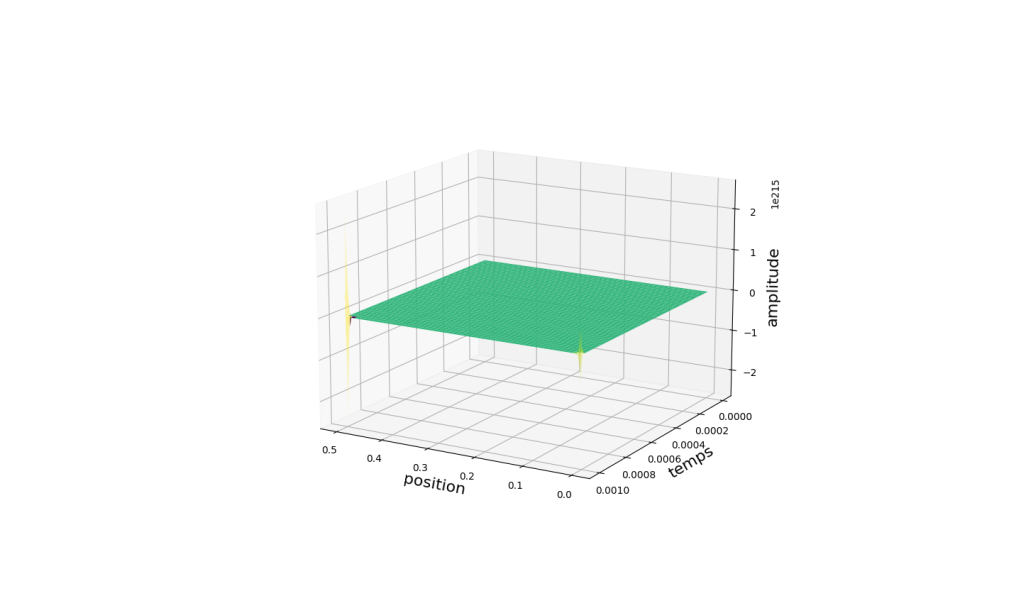
\includegraphics[width=12cm,height=6cm]{explicited.png}

\end{minipage}%

\begin{minipage}{.5\textwidth}%

\item $\Delta x$ = $5*{10}^{-4}m$\\
$\Delta t$=${10}^{-6} s $ \\
$\lambda$=$6,8*{10}^{-1}s$\\

$\Longrightarrow$ On obtient une courbe parfaitement sinusoïdale.\\
Temps d'exécution = $1,24s$

\end{minipage}%
\hfill
\begin{minipage}{.45\textwidth}%
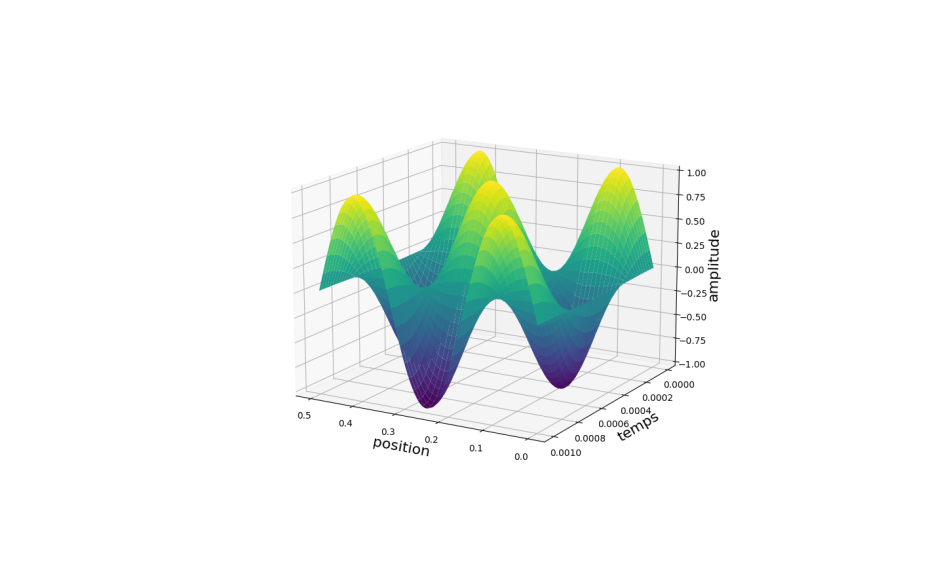
\includegraphics[width=12cm,height=6cm]{explicitee.png}

\end{minipage}%

\begin{minipage}{.5\textwidth}%


\item $\Delta x$=$5*{10}^{-4}m$\\
$\Delta t={10}^{-8}$\\
$\lambda$=$6,8*{10}^{-3}s$\\


$\Longrightarrow$ On obtient une courbe parfaitement sinusoïdale.\\
Temps d'exécution =$122s$
\end{minipage}%
\hfill
\begin{minipage}{.45\textwidth}%
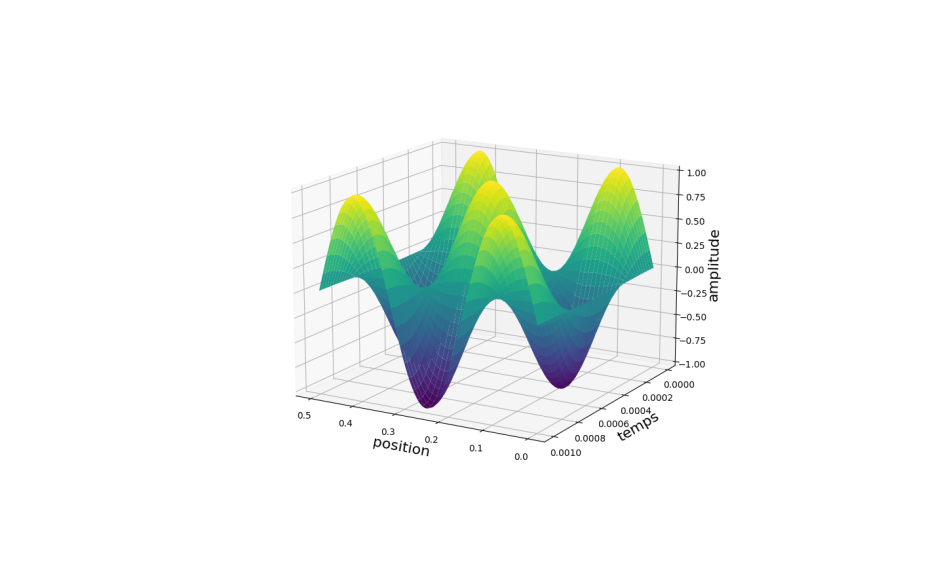
\includegraphics[width=12cm,height=6cm]{explicitee.png}
\end{minipage}%



\end{enumerate}
D'après ces différents tests, on peut remarquer que le schéma est de plus en plus sinusoïdale lorsque le CFL se rapproche de 1.\\



$\triangleright$\textbf{Variation de  $\Delta x$ à $\Delta t$ fixé :}\\

On fixe $\Delta t$ à différentes valeurs:\\

\hspace*{1cm}$\bullet$ Pour $\Delta t= {10}^{-3}$ \\

\begin{enumerate}[label=\alph*)]

\begin{minipage}{.6\textwidth}%

\item $\Delta x=3,4*{10}^{-2}m$ \\
$\Delta t= {10}^{-4}$ \\
$\lambda= 1$\\


$\Longrightarrow$ On obtient aucun affichage.

\end{minipage}%
\hfill
\begin{minipage}{.6\textwidth}%

\item $\Delta x=7*{10}^{-2}m$ \\
$\Delta t= {10}^{-4}$ \\
$\lambda= 4,8*{10}^{-1}m$\\


$\Longrightarrow$ On obtient aucun affichage.\\

\end{minipage}%


\end{enumerate}

\vspace*{1cm}
\hspace*{1cm}$\bullet$ Pour $\Delta t= {10}^{-6}$ \\

\begin{enumerate}[label=\alph*)]

\begin{minipage}{.45\textwidth}%

\item $\Delta x=4*{10}^{-3}m$ \\
$\Delta t= {10}^{-6}$ \\
$\lambda= 0,85$\\


$\Longrightarrow$ On obtient la représentation d'une onde parfaitement sinusoïdale.\\
Temps d'exécution = $0,043s$

\end{minipage}%
\hfill
\begin{minipage}{.6\textwidth}%
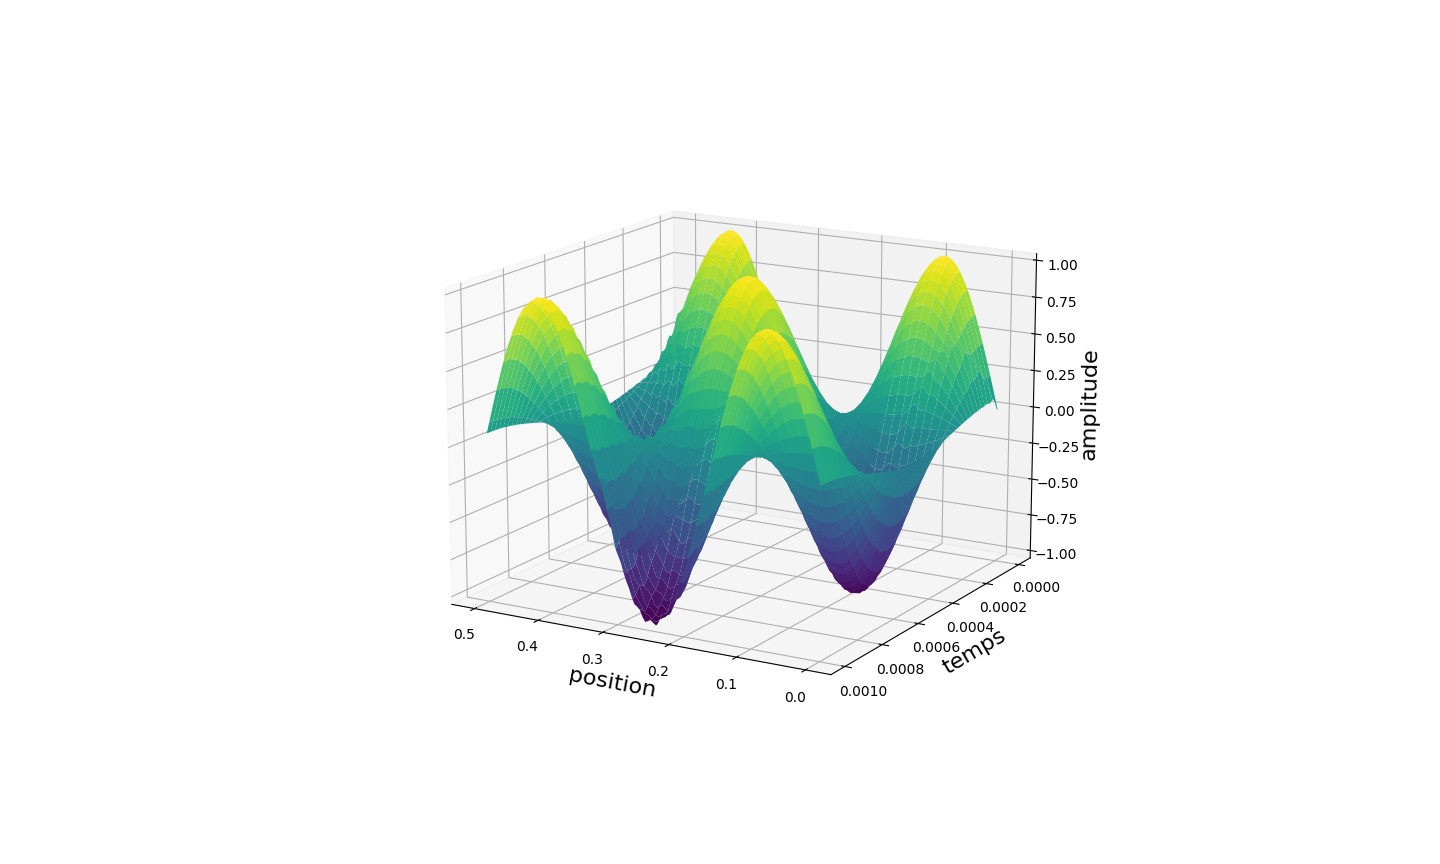
\includegraphics[width=12cm,height=6cm]{dt=10^-6 et dx=0.004.png}

\end{minipage}%
\newline
\begin{minipage}{.45\textwidth}%
\item $\Delta x=4*{10}^{-2}m$ \\
$\Delta t= {10}^{-6}$ \\
$\lambda= 0,0085$\\


$\Longrightarrow$ On obtient une figure sinusoïdale.\\
Temps d'exécution = $0,016s$

\end{minipage}%
\begin{minipage}{.45\textwidth}%
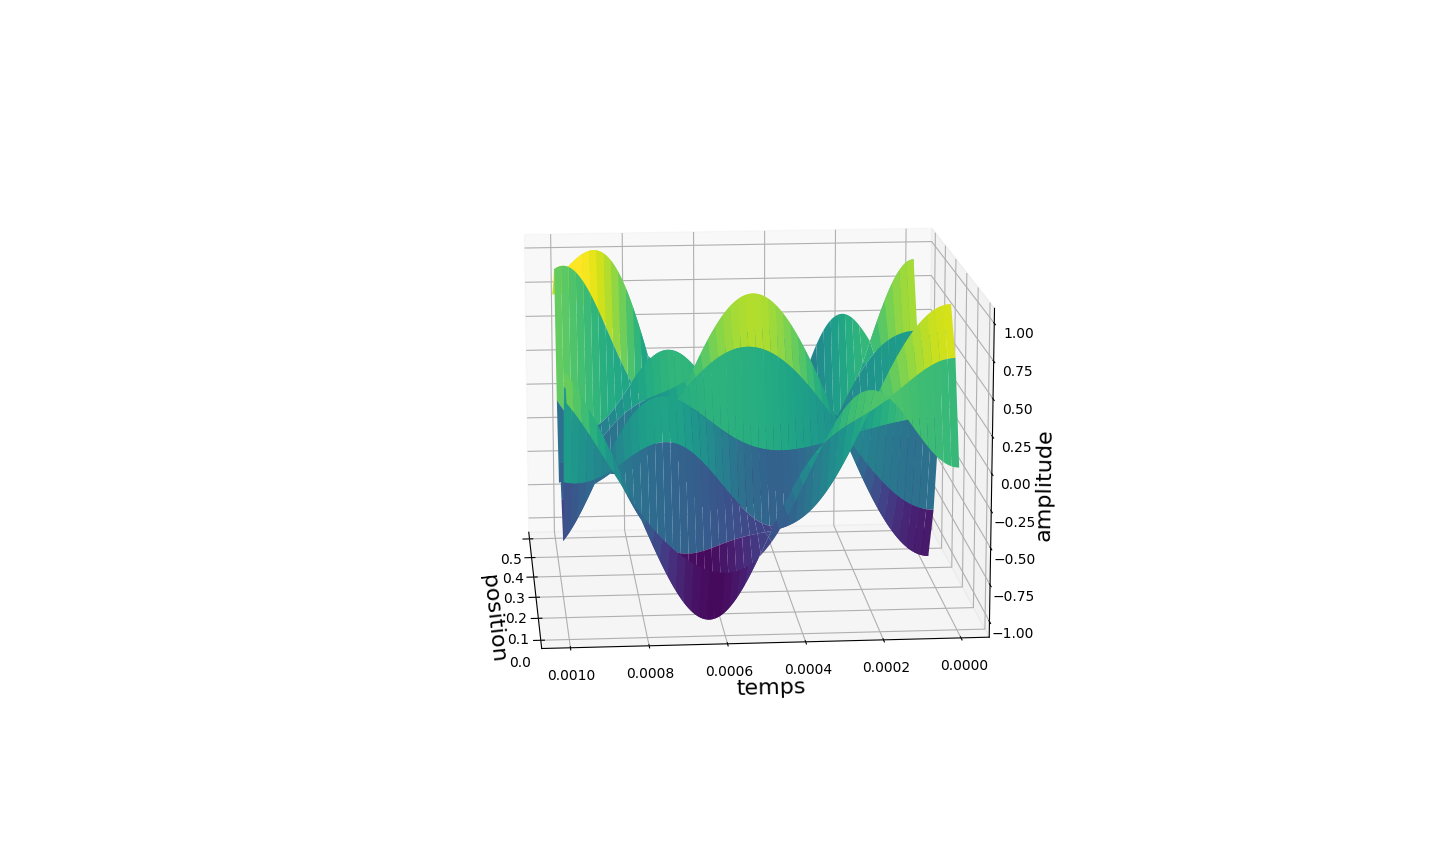
\includegraphics[width=12cm,height=6cm]{dt=10^-6 avec dx=0.04.png}

\end{minipage}%

On constate à travers ces différents tests concernant la variation de l'espace à $\Delta t$ fixé, que les représentations se modélisent de mieux en mieux lorsque notre $\Delta t$ décroît.


\end{enumerate}


\subsubsection{Schéma implicite :}

$\triangleright$ \textbf{Variation de $\Delta t$ (en secondes) à $\Delta x$ (en mètres) fixé :}\\
\begin{enumerate}[label=\alph*)]


\begin{minipage}{.5\textwidth}%

\item $\Delta x =  5*{10}^{-4}m$\\
$\Delta t$ = ${10}^{-2} s $\\
$\lambda$ =$6,8*{10}^{3}$\\

$\Longrightarrow$ Représentation non supportée donc aucun affichage car $\lambda$ est trop grand.\\ 

\end{minipage}%




\begin{minipage}{.5\textwidth}%
\item $\Delta x = 5*{10}^{-4}m $\\
$\Delta t$ = ${10}^{-4}m s $ \\
$\lambda =68$ \\

$\Longrightarrow$ En ayant un $\lambda$ qui se rapproche de 1, on obtient une onde partiellement sinusoïdale.\\
Temps d'exécution = $0,207s$

\end{minipage}%
\hfill
\begin{minipage}{.45\textwidth}%
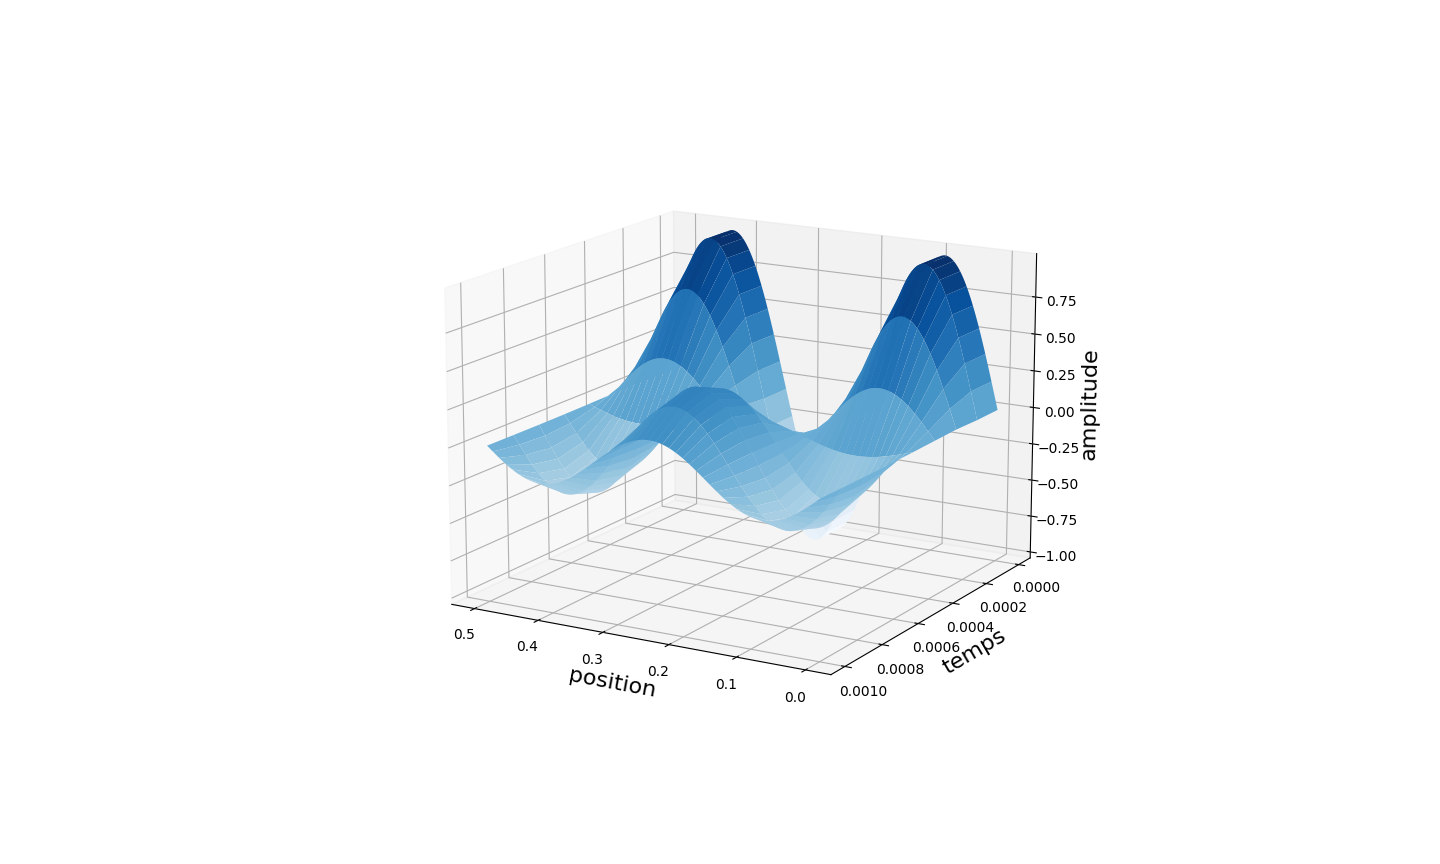
\includegraphics[width=10cm,height=6cm]{implicitec.png}
\end{minipage}%

\begin{minipage}{.5\textwidth}%
\item $\Delta x = 5*{10}^{-4}m$\\
$\Delta t$ = ${10}^{-5} s $ \\
$\lambda =6,8$\\

$\Longrightarrow$ On obtient une surface parfaitement  sinusoïdale lorsque le pas de temps est plus petit et donc par conséquent un $\lambda$ plus petit se rapprochant de 1.\\ 
Temps d'exécution = $0,302s$
\end{minipage}%
\hfill
\begin{minipage}{.45\textwidth}%
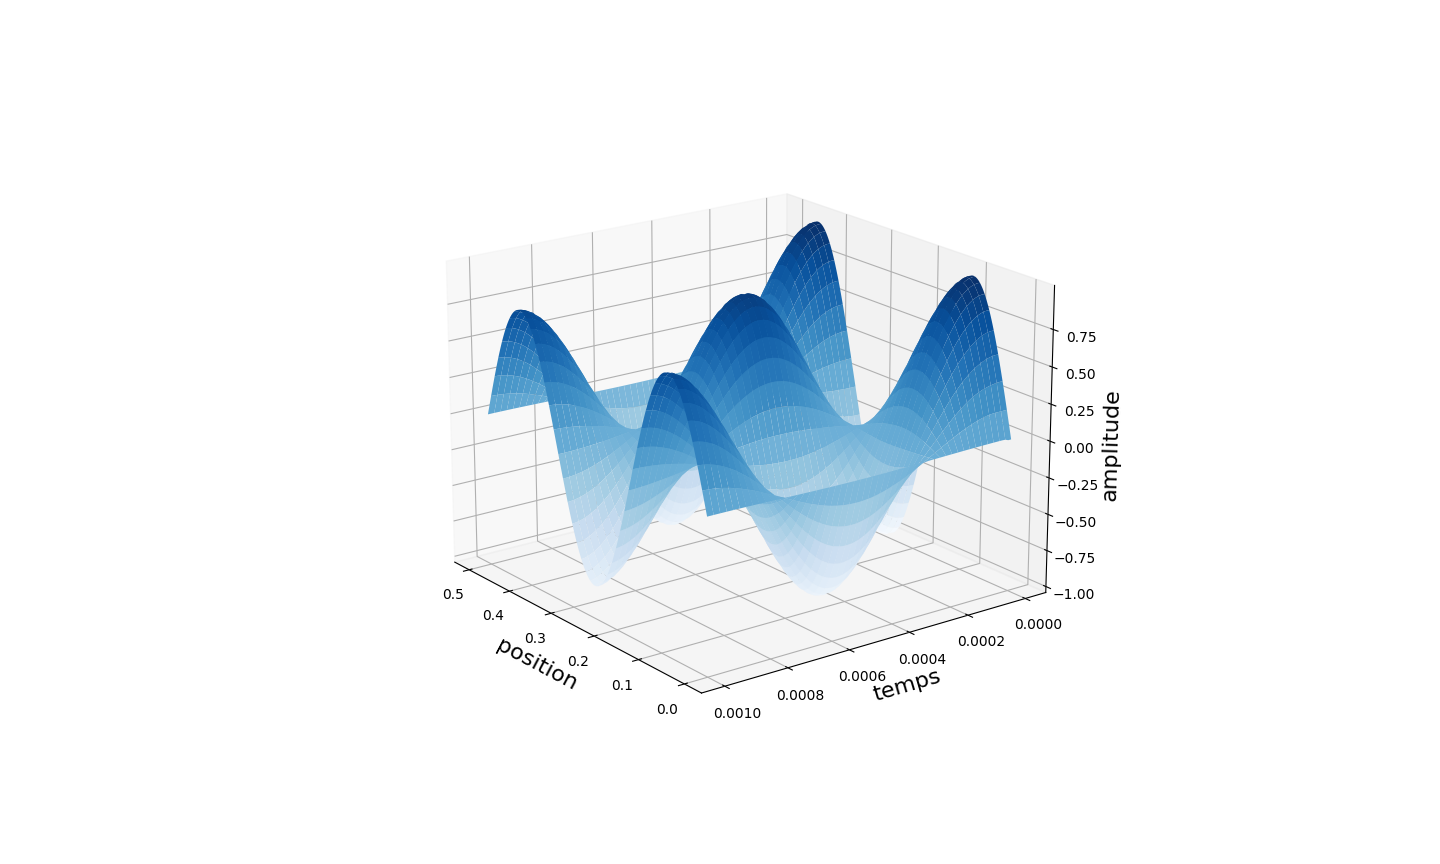
\includegraphics[width=10cm,height=6cm]{implicited.png}
\end{minipage}%




\begin{minipage}{.8\textwidth}%

\item $\Delta x=5*{10}^{-4}m$\\
$\Delta t$=${10}^{-8}$\\
$\lambda$=$6,8*{10}^{-3}s$\\


$\Longrightarrow$On obtient aucune représentation de l'onde car le pas de $\lambda$ est trop petit.\\

\end{minipage}%
\newline
\newline
Le coefficient CFL joue un rôle très important dans la stabilité du modèle, ce dernier liant les pas de temps et d'espace nous permet d'avoir des représentations plus ou moins sinusoïdales en fonction de la variation de $\Delta t$.
\end{enumerate}

$\triangleright$\textbf{Variation de  $\Delta x$ à $\Delta t$ fixé :}\\

\begin{enumerate}[label=\alph*)]

\hspace*{1cm}$\bullet$ Pour $\Delta t= {10}^{-3}$ \\
\newline

\begin{minipage}{.6\textwidth}%

\item $\Delta x=5*{10}^{-3}m$ \\
$\Delta t= {10}^{-3}$ \\
$\lambda= 680$\\


$\Longrightarrow$ On obtient aucun affichage.

\end{minipage}%

\begin{minipage}{.45\textwidth}%

\item $\Delta x=3*{10}^{-2}m$ \\
$\Delta t= {10}^{-5}$ \\
$\lambda= 1,1*{10}^{-1} $\\


$\Longrightarrow$ On commence à avoir une forme d'onde sinusoïdale. 

\end{minipage}%
\hfill
\begin{minipage}{.6\textwidth}%
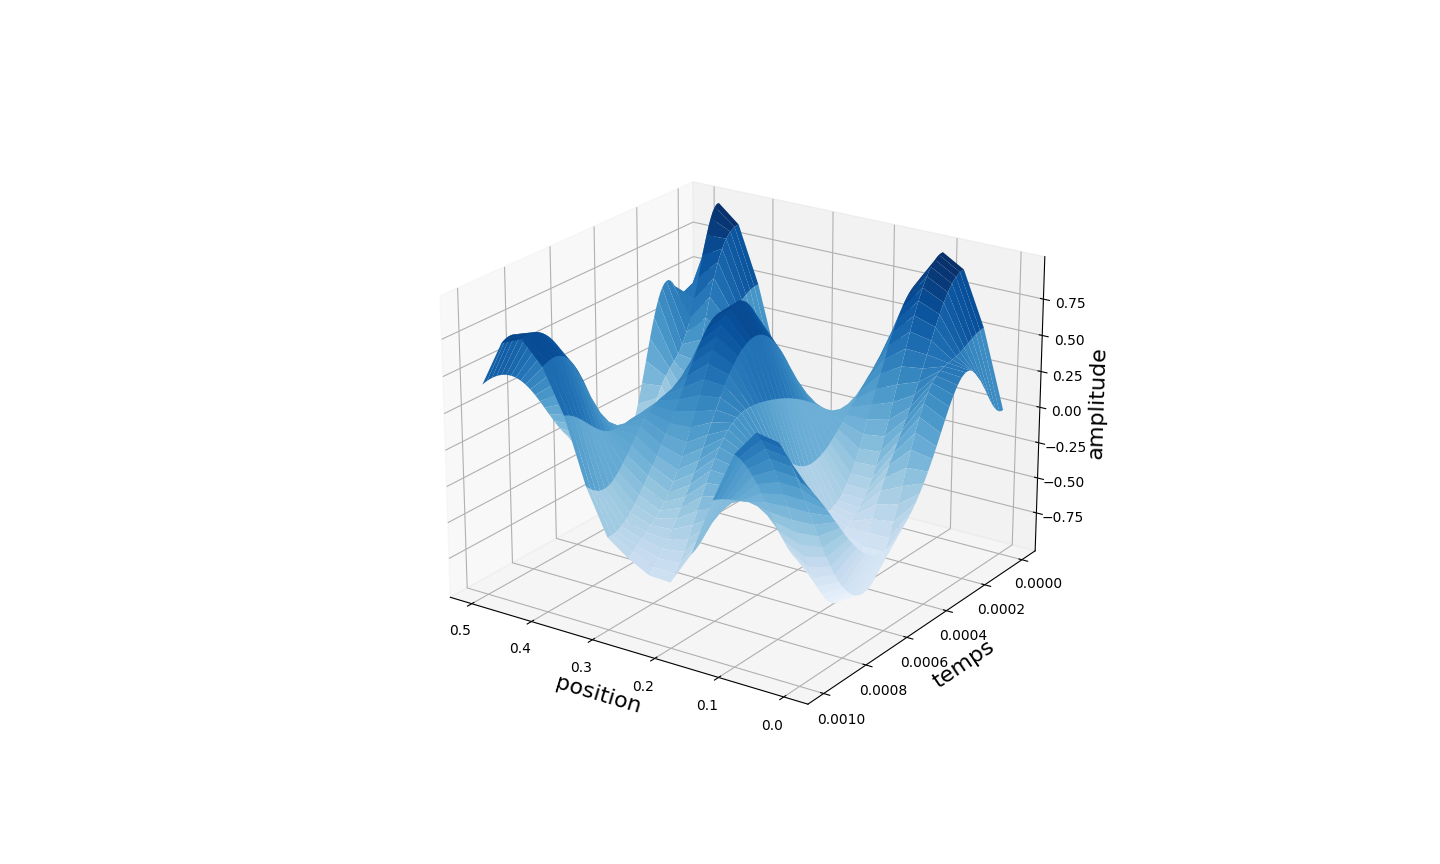
\includegraphics[width=12cm,height=6cm]{dt=0.00001 avec dx=0.03.png}
\end{minipage}%


\hspace*{1cm}$\bullet$ Pour $\Delta t= {10}^{-5}$ \\

\begin{minipage}{.45\textwidth}%
\item $\Delta x=9*{10}^{-2}m$\\
$\Delta t={10}^{-5}$\\
$\lambda= 0,03$ \\
$\Longrightarrow$ L'onde commence à apparaître de maniére imprécise.
\end{minipage}%
\hfill
\begin{minipage}{.6\textwidth}%
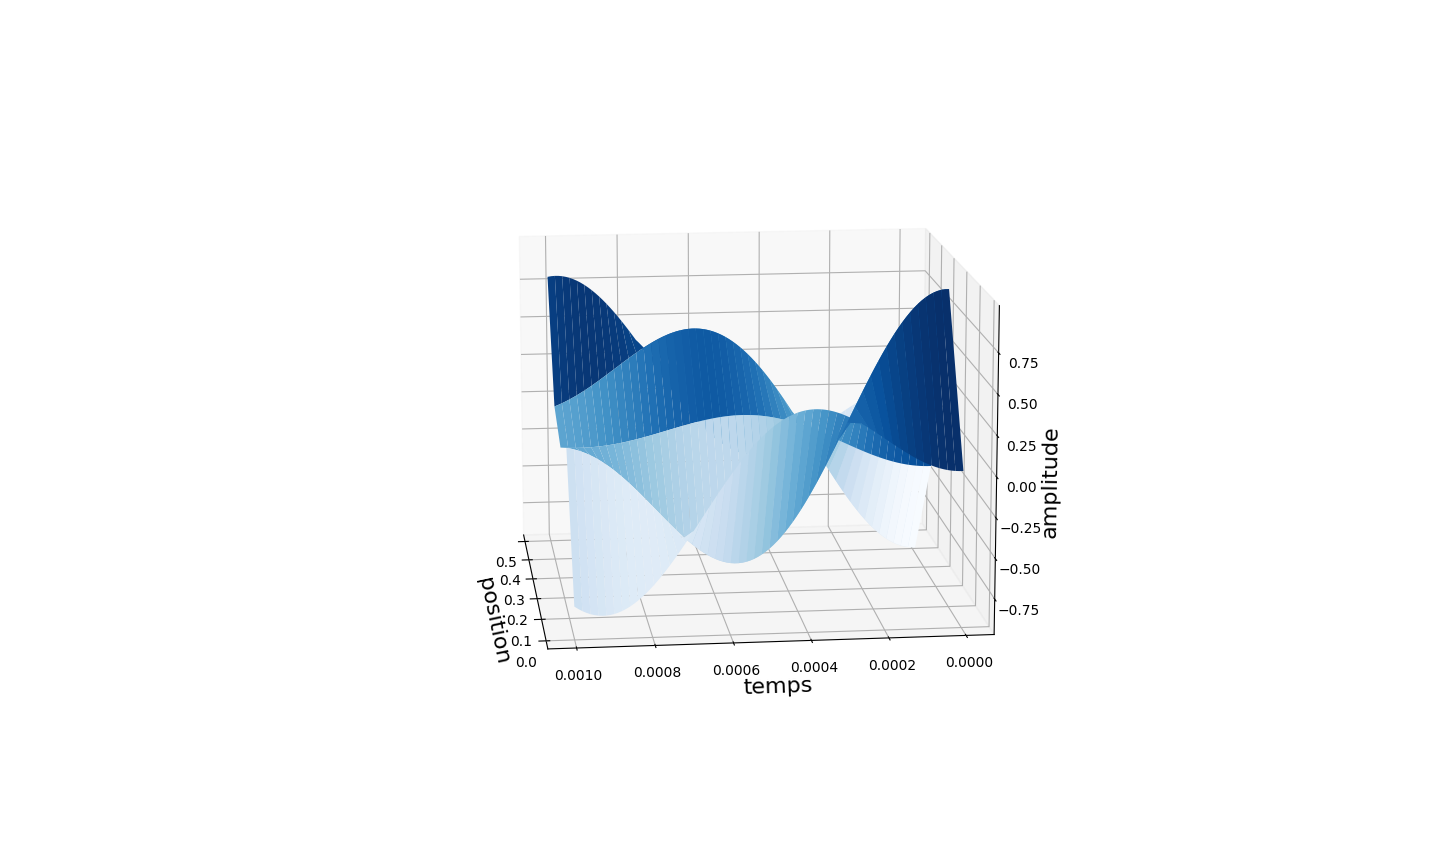
\includegraphics[width=12cm,height=6cm]{dt=0.00001 et dx=0.09.png}
\end{minipage}%

\hspace*{1cm}$\bullet$ Pour $\Delta t= {10}^{-6}$ \\
\begin{minipage}{.45\textwidth}%

\item $\Delta x=7*{10}^{-3}m$ \\
$\Delta t= {10}^{-6}$ \\
$\lambda=0,048s $\\


$\Longrightarrow$ On obtient une représentation parfaitement sinusoïdale.

\end{minipage}%
\hfill
\begin{minipage}{.6\textwidth}%

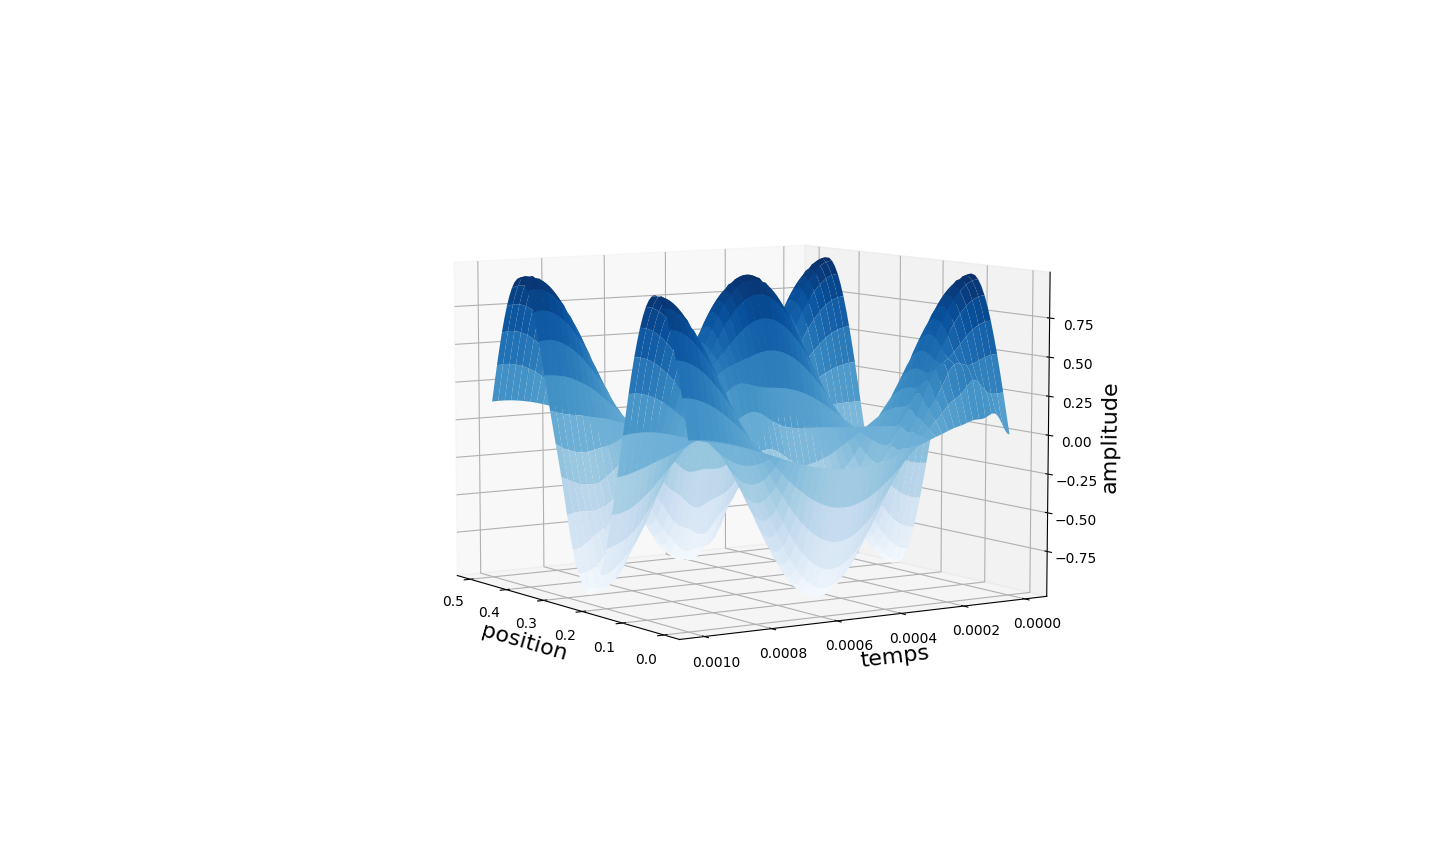
\includegraphics[width=12cm,height=6cm]{dt=10^-6 avec dx= 0.007 .png}
\end{minipage}

\begin{minipage}{.45\textwidth}%

\item $\Delta x=2,4*{10}^{-2}m$ \\
$\Delta t= {10}^{-6}$ \\
$\lambda=1,4*{10}^{-2} $\\


$\Longrightarrow$ On a une représentation sinusoïdale. 
\end{minipage}%
\hfill
\begin{minipage}{.6\textwidth}%

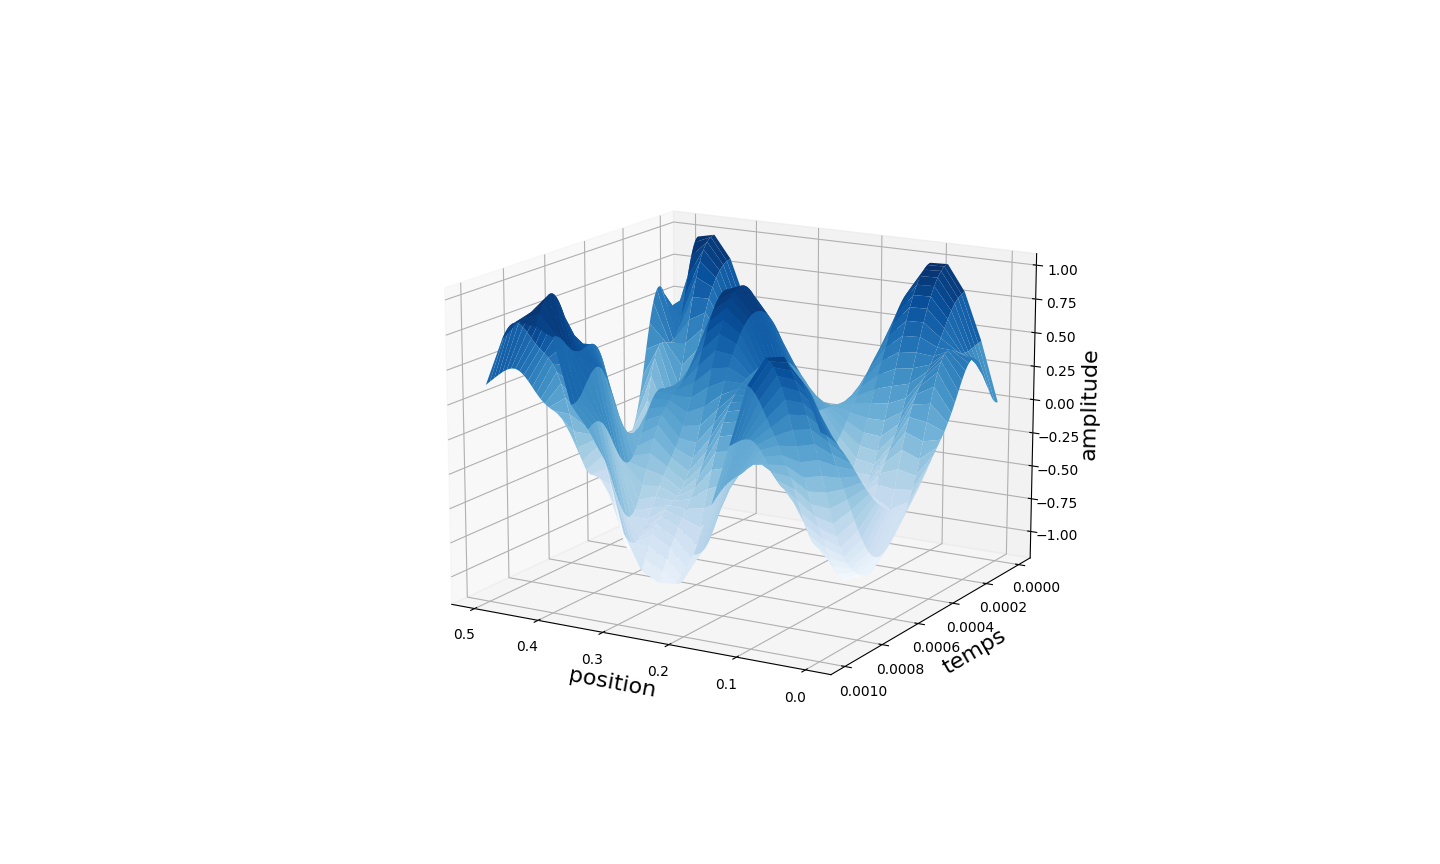
\includegraphics[width=12cm,height=6cm]{dt=10^-6 avec dx=0.024.png}
\end{minipage}
On obtient comme précédemment, une modélisation représentative de l'onde lorsque le pas de temps diminue mais également en ayant un pas d'espace d'ordre ${10}^{-2}$\\


\textbf{Conclusion}: On peut remarquer d'après cette série de tests, que la stabilité est obtenu généralement avec un coefficient CFL proche de 1 par conséquent un pas d'espace $\Delta x$ de l'ordre ${10}^{-2}$ au minimum et un pas de temps de l'ordre ${10}^{-5}$ au minimum.   


\end{enumerate}

\subsection{Méthode de Runge-Kutta}
Le principe d'étude de la stabilité du modèle reste le même que pour les schémas d'Euler. Il faut donc faire varier les pas $\Delta x$ et $\Delta t$ de manière à avoir les meilleurs graphiques.
Mais, il apparaît assez évident que le modèle risque de diverger avec le terme $(\frac{c}{\Delta x})^2$.\\

    
\begin{figure}[H]
\begin{minipage}[b]{.46\linewidth}
\centering\epsfig{figure=33.png,width=7cm}
\caption{
        $\Delta x= 5^{-3}m $\\
        $\Delta t= 10^{-4}s$\\
        $\lambda = 6.8$
    \label{fig1}
    }
\end{minipage} \hfill
\begin{minipage}[b]{.46\linewidth}
\centering\epsfig{figure=11.png,width=7cm}
\caption{$\Delta x= 5^{-3}m $\\ 
        $\Delta t= 10^{-5}s$\\
        $\lambda = 0.68$
        \label{fig2}}
\end{minipage}
\end{figure}

\begin{figure}[H]
\begin{minipage}[b]{.46\linewidth}
\centering\epsfig{figure=6.png,width=7cm}
\caption{$\Delta x= 5^{-2}m $\\ 
        $\Delta t= 10^{-6}s$\\
        $\lambda = 0.0068$
        \label{fig1}}
\end{minipage} \hfill
\begin{minipage}[b]{.46\linewidth}
\centering\epsfig{figure=8.png,width=\linewidth}
\caption{$\Delta x= 5^{-3} m $\\ 
        $\Delta t= \frac{\Delta x}{c}s= 1.47.10^{-5} $\\
        $\lambda = 1$
        \label{fig2}}
\end{minipage}
\end{figure}


A partir des simulations effectuées (les autres étant en annexe 5), est possible d'observer expérimentalement les conditions de stabilité du modèle construit.
\begin{enumerate}
    \item Par rapport au CFL : $\lambda = c\frac{\Delta t}{\Delta x}$\\
    On peut remarquer que le modèle est "correct" uniquement lorsque $\lambda < 1 $  (Figure 2).\\
    Dans les autres cas, le résultat est loin de ce qui attendu. Cela est logique étant donné qu'il s'agit ici d'une méthode à deux pas, donc le CFL est un paramètre important.
    \item Par rapport aux valeurs  de $\Delta t$ et $\Delta x$ \\
    On peut logiquement remarquer que la stabilité du modèle augmente lorsque le pas $\Delta t$ diminue, il faut que $\Delta t$ soit plus petit que $\Delta x$ et que $\Delta x$ soit assez petit mais trop le diminuer ferait diverger le modèle.\\
    Cela découlerait du facteur $(\frac{c}{\Delta x})^2$ qui augmente énormément lorsque $\Delta x$ diminue.
    
\end{enumerate}


\section{Comparaison des méthodes}
L'objectif principal du projet est de comparer les différentes méthodes de résolution numérique pour l'équation d'onde appliquée à une corde de guitare.
Pour cela, nous allons comparer expérimentalement les erreurs obtenues pour chaque modèle pour des conditions de stabilité optimales et pour une solution exacte donnée.

\subsection{Étude des erreurs}
Pour effectuer les calculs d'erreurs, nous avons choisi la fonction suivante :
\begin{equation*}
    u_{exact}(x,t)=cos(\frac{3 \pi c}{L}t)sin(\frac{3 \pi }{L}x )
\end{equation*}
Et donc l'erreur numérique est simplement donnée par :
     $E=|u_{exact} - u_{num}|$

Ainsi, on obtient comme conditions initiales pour les trois modèles:
  \[
      \begin{cases}
        u^{0}_{i}=\sin(\frac{n \pi }{L} \times i \times \Delta x) \\
        \frac{\partial u^0_{i}}{\partial t}= 0
      \end{cases}
    \]\\
Et les paramètres des modèles sont les suivants:
\begin{itemize}
    \item $c$=340 m/s (vitesse arbitraire mais qui correspond à la vitesse d'une onde dans l'air)
    \item $L$=0.5 m (longueur moyenne d'une corde de guitare)
    \item $Durée$=0.001 s\\ 
\end{itemize}
Et les paramètres de discrétisation pour les méthodes d'Euler sont:
\begin{itemize}
    \item $\Delta x=0.0005$
    \item $\Delta t=\frac{\Delta x}{c}$
\end{itemize}
Ceux de la méthode de Runge-Kutta sont: 
\begin{itemize}
    \item $\Delta x=0.005$
    \item $\Delta t=0.000001$
\end{itemize}

L'on pourra retrouver les graphiques des solutions pour ces 4 méthodes de calcul en annexe 2.


On peut déjà remarquer que pour les 3 modèles, les solutions numériques sont très proches de la solution exacte en terme de forme de surface mais aussi en terme d'amplitude.


Voici les résultats donnés par les calculs d'erreurs numériques en 3 dimensions.
\begin{figure}[H]
\begin{minipage}[b]{.46\linewidth}
\centering\epsfig{figure=1_comp.png,width=7cm}
\caption{Euler explicite
    \label{fig1}
    }
\end{minipage} \hfill
\begin{minipage}[b]{.46\linewidth}
\centering\epsfig{figure=2_comp.png,width=7cm}
\caption{Euler implicte\label{fig2}}
\end{minipage}
\end{figure}


\begin{figure}[H]
\begin{center}
\begin{minipage}[b]{.46\linewidth}
\centering\epsfig{figure=3_comp.png,width=7cm}
\caption{Runge-Kutta\label{fig1}}
\end{minipage} \hfill
\end{center}
\end{figure}

Les erreurs pour chaque modèle prennent des formes différentes.
Pour les méthodes d'Euler, on peut observer des structures "sinusoïdales" quasiment périodiques. On peut cependant observer sur le schéma explicite une diminution générale de l'erreur à partir d'une certaine position.
Pour le schéma de Runge-Kutta, on retrouve une forme similaire à celle de la méthode d'Euler explicite avec également la même diminution de l'erreur.
\newline
Mais il est plus intéressant d'évaluer les erreurs en 2 dimensions selon le temps. Ainsi, nous avons étudié les moyennes des erreurs pour chaque temps donné.
\newline
Les moyennes des erreurs pour chaque t donnés nous donnent alors les graphiques suivants:

\begin{figure}[H]
\begin{center}
\centering\epsfig{figure=7.comp.png,width=15cm}
\caption{Les erreurs pour les 3 méthodes\label{fig1}}
\end{center}
\end{figure}

Les erreurs en fonction de t nous permettent de voir que le modèle le plus précis est le modèle d'Euler explicite.
Globalement les erreurs ont bien des profils sinusoïdaux mais elles augmentent en fonction du temps, ce qui montre que les modèles présentent des facteurs de propagation d'erreur.
Le modèle le moins précis est le modèle de Runge-Kutta.
L'ordre des erreurs est de $10^-2$ pour les modèles mais le modèle de Runge-Kutta a une erreur qui croît beaucoup plus vite.

\vspace{1cm}
\subsection{Ordre des erreurs}
Pour finir la comparaison des modèles, nous pouvons déterminer et comparer l'ordre de leurs erreurs.
Pour cela, nous pouvons étudier les expressions suivantes:
\begin{enumerate}
    \item $max|e^n_{i}|$ pour $0<i<Nx$ et $0<n<Nt$ en faisant varier le nombre de point de temps $Nt$ (Figure 9)
    \item $max|e^n_{i}|$ pour $0<i<Nx$ et $0<n<Nt$ en faisant varier le nombre de point d'espace $Nx$ (Figure 10)
\end{enumerate}

Voici les résultats obtenus:

\begin{figure}[H]
\begin{center}
\centering\epsfig{figure=erreur_dt.png,width=15cm}
\caption{Les erreurs pour des variation de $Nt$\label{fig1}}
\end{center}
\end{figure}

\begin{figure}[H]
\begin{center}
\centering\epsfig{figure=erreurs_dx.png,width=15cm}
\caption{Les erreurs pour des variation de $Nx$\label{fig1}}
\end{center}
\end{figure}

A partir de ces résultats, on peut déduire les ordres des erreurs:
\begin{itemize}
    \item Les méthodes d'Euler ont des erreurs selon $x$ et $t$ d'ordre $O(N)$
    \item La méthode de Runge-Kutta a des erreurs  d'ordre $O(N^2)$ puis constante selon $t$ et d'ordre $O(N)$ selon $x$.On peut déjà remarquer que la précision n'augmente plus en diminuant $\Delta t$ à partir d'une certaine valeur. On peut également remarquer que selon $x$, l'erreur augmente brutalement au bout d'une certaine valeur, cela est dû au fait que la condition de stabilité du modèle n'est plus respectée. On peut remarquer grâce
    \item Globalement la méthode d'Euler explicite est celle qui donne la meilleure précision.
\end{itemize}

Au final, on peut déduire que, dans notre cas, la méthode d'Euler explicite est la plus intéressante puisqu'elle produit l'erreur la plus petite mais est également efficace en terme d'algorithme contrairement à la méthode de Runge-Kutta qui demande beaucoup plus de calculs pour avoir un résultat cohérent.



\section{Conditions initiales}

\subsection{Variation des conditions initiales}


L'analyse des méthodes utilisées pour la modélisation d'une onde  de corde de guitare repose aussi sur le choix des conditions initiales comme vu précédemment.
Un bon choix des conditions initiales est donc indispensable pour avoir une modélisation la plus proche de la réalité ou tout simplement celle qu'on souhaite.\\


Dans cette partie, l'objectif est de tester les différents schémas pour différents profils initiaux de l'onde, que l'on obtiendra en modifiant les conditions initiales. \\

Ainsi, on pourra visualiser les réactions des différents modèles par rapport aux variations de conditions initiales et constater que, tant que les conditions initiales respectent les conditions imposées par le problème $(u(t,x=0)=u(t,x=L)=0)$, on obtient une solution numérique cohérente.\\

Dans un premier temps, on peut considérer une corde pincée en point de l'espace, qui est bien attachée sur les bords.
On peut établir 2 modèles mathématiques différents pour la corde pincée du schéma suivant:

\begin{figure}[H]
\centering
\includegraphics[scale=1]{image2.png}
\caption{Schéma d'une corde pincée}
\label{fig1}
\end{figure}



\begin{enumerate}
    \item Modèle triangulaire
    \begin{equation}
       u(x,t=0)=\left\{
            \begin{array}{ll}
               \ A \frac{x}{x_{0}} &  x\leq x_{0} \\
               \ A \frac{x}{x_{0}} &  x\leq x_{0}
            \end{array}
        \right.
    \end{equation}
    
    
    \item Modèle complet (harpe)
    \begin{equation}
        u(x,t=0)=A\frac{x}{x_{0}}\frac{L-x}{L}
    \end{equation}
    
Dans un deuxième temps, nous allons étudier un troisième modèle où la corde n'est pas accrochée aux bords, c'est-à-dire que, $u(t=0,x=0)$ on a une amplitude $A$ différente de $0$. Le résultat ne devrait alors pas être correct étant donné qu'il ne respecte plus les conditions du problème.
\newline

 \item Modèle "non accroché aux bords"
    \begin{equation}
       \left\{
            \begin{array}{ll}
               \  u(x,t=0)=cos(\frac{n \pi x}{L})  \\
               \ \frac{\partial{u}}{\partial{t}}(x,t=0)=0 
            \end{array}
        \right.
    \end{equation}
    
    
    
    
    
    
\end{enumerate}


\vspace*{2cm}
\subsection{Implémentation des variations des conditions initiales dans les modèles}


\underline{Méthode d'Euler explicite}



\begin{figure}[H]
\minipage{0.32\textwidth}
  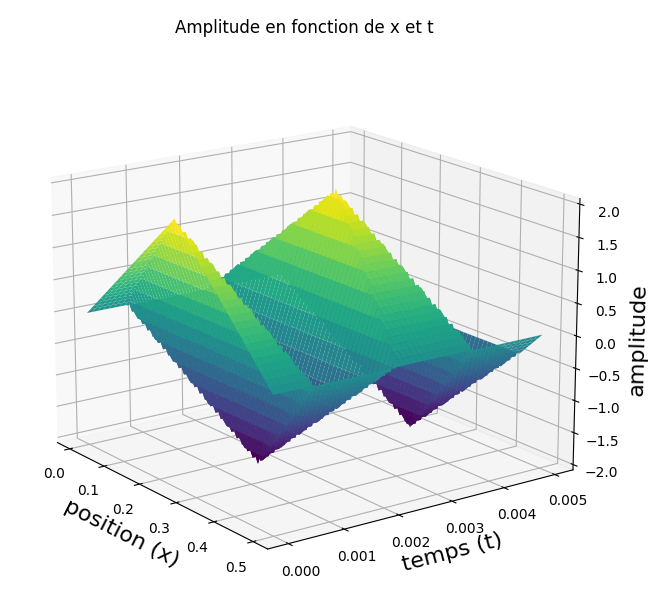
\includegraphics[width=5cm]{1.png}
  \caption{Modèle (1)}\label{fig}
\endminipage\hfill
\minipage{0.32\textwidth}
  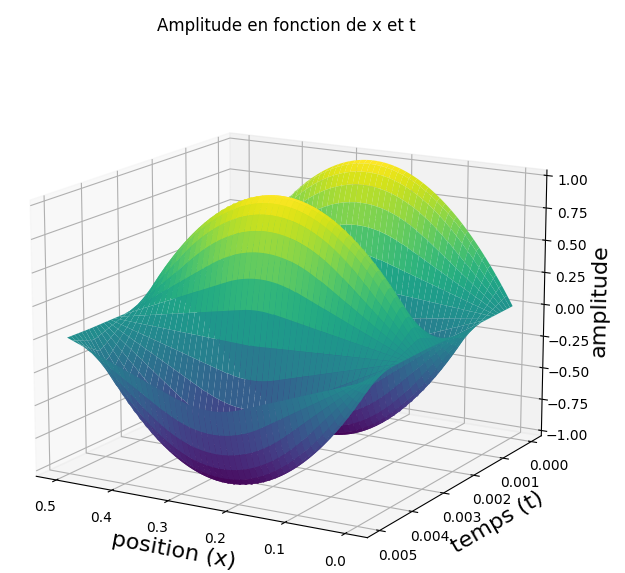
\includegraphics[width=5cm]{2.png}
  \caption{Modèle (2)}\label{fig}
\endminipage\hfill
\minipage{0.32\textwidth}%
  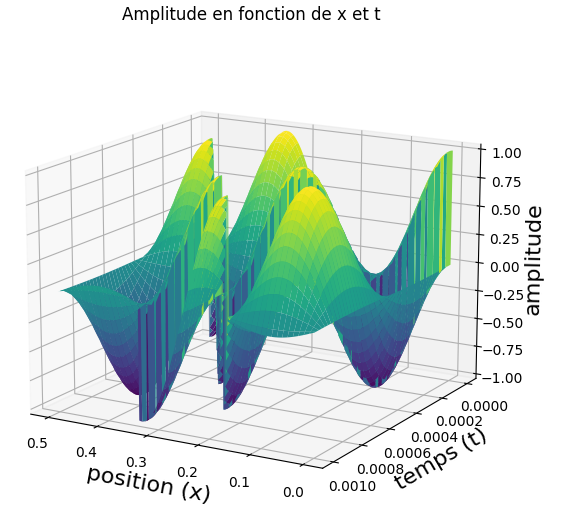
\includegraphics[width=5cm]{7_explicite.png}
  \caption{Modèle (3)}\label{fig}
\endminipage
\end{figure}



\underline{Méthode d'Euler implicite}

\begin{figure}[H]
\minipage{0.32\textwidth}
  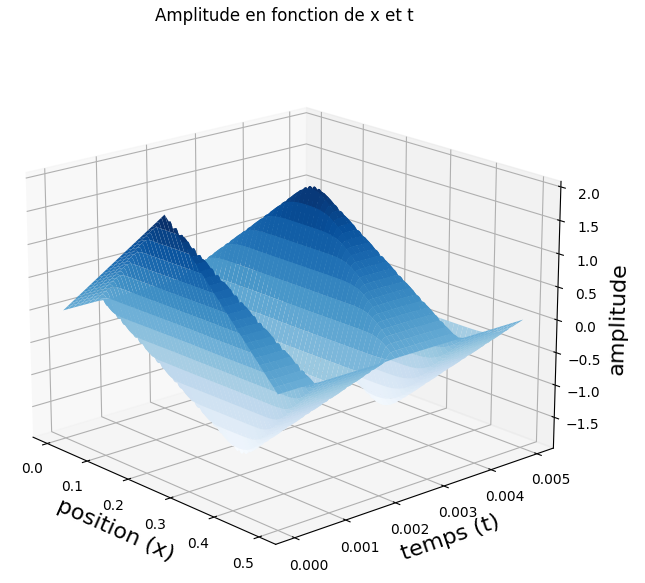
\includegraphics[width=5cm]{3.png}
  \caption{Modèle (1)}\label{fig}
\endminipage\hfill
\minipage{0.32\textwidth}
  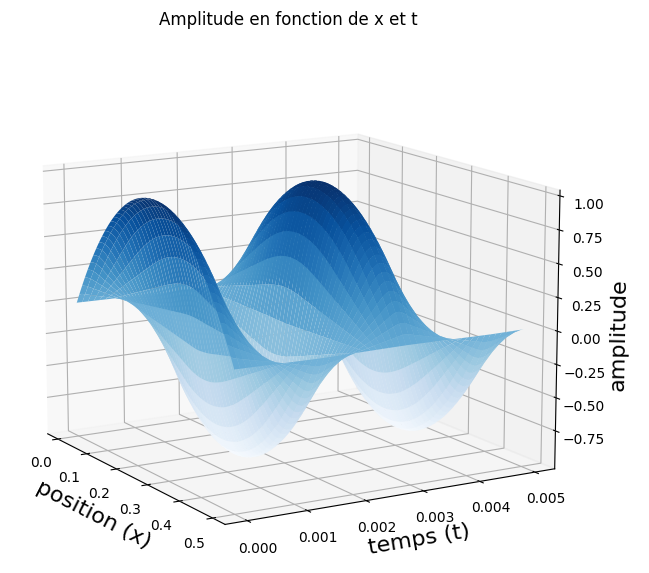
\includegraphics[width=5cm]{4.png}
  \caption{Modèle (2)}\label{fig}
\endminipage\hfill
\minipage{0.32\textwidth}%
  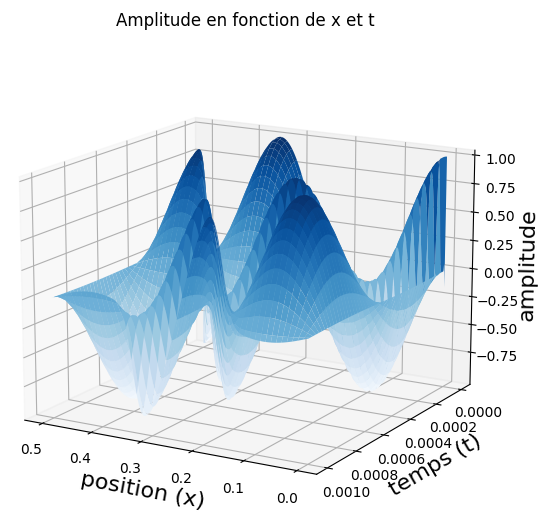
\includegraphics[width=5cm]{8_implicite.png}
  \caption{Modèle (3)}\label{fig}
\endminipage
\end{figure}


\underline{Méthode de Runge-Kutta}
   
\begin{figure}[H]
\minipage{0.32\textwidth}
  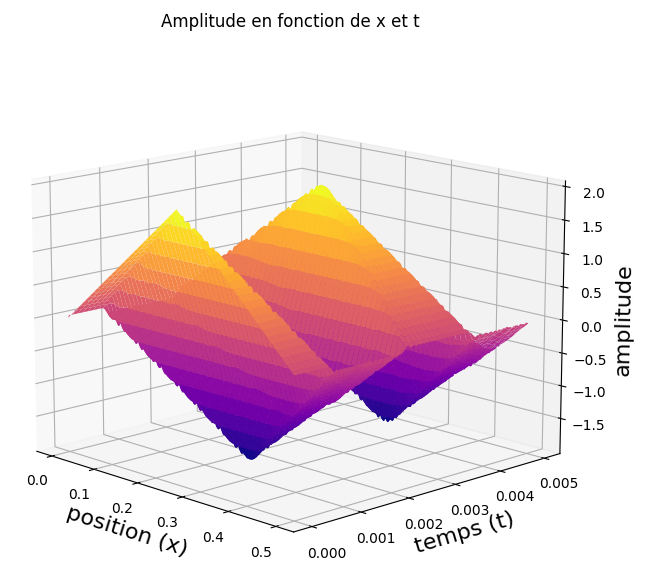
\includegraphics[width=5cm]{5.png}
  \caption{Modèle (1)}\label{fig}
\endminipage\hfill
\minipage{0.32\textwidth}
  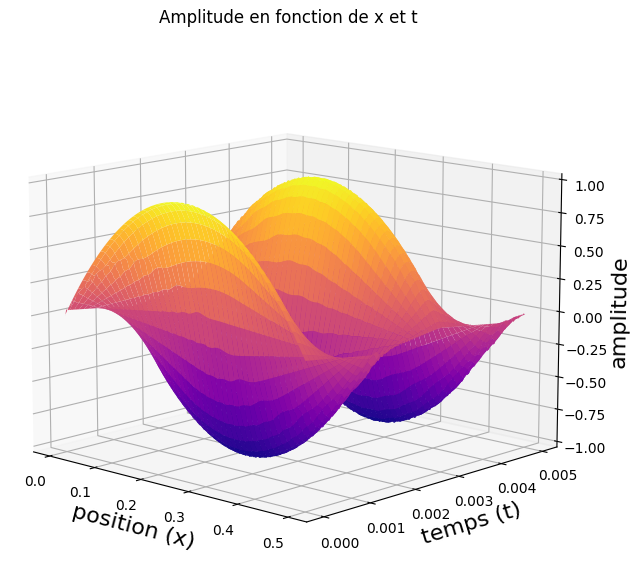
\includegraphics[width=5cm]{6_pro.png}
  \caption{Modèle (2)}\label{fig}
\endminipage\hfill
\minipage{0.32\textwidth}%
  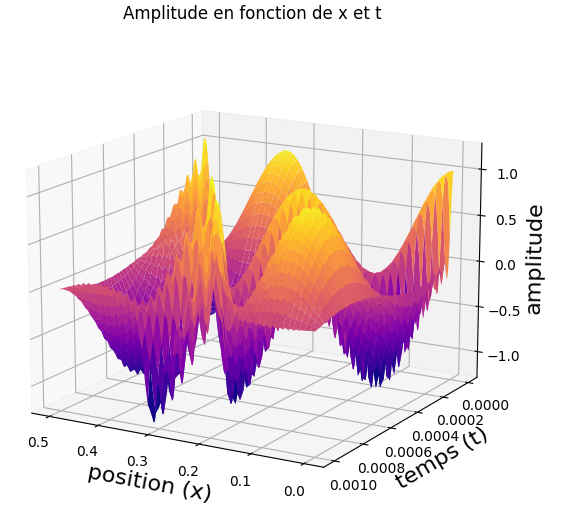
\includegraphics[width=5cm]{9_RK.png}
  \caption{Modèle (3)}\label{fig}
\endminipage
\end{figure}


\part{Conclusion}

\section{Conclusion du projet}
Au cours de ce projet, nous voulions réaliser des modèles propagation des ondes dans un instrument à corde afin de les comparer. Nous avons pu établir 3 modèles différents pour résoudre numériquement l'équation d'onde. Ces modèles mathématiques permettent d'obtenir des solutions numériques relativement proche de la solution exacte.
Nous pouvons résumer les points importants de chaque méthode:
\begin{itemize}
    \item Euler explicite : efficacité de calcul avec une formule de récurrence,utilisation de la vectorialisation (numpy) et précision à $10^-2$
    \item Euler implicite : efficacité de calcul avec résolution de système,utilisation de vectorialisation (numpy) et précision à $10^-2$
    \item Runge-Kutta : méthode non efficace à cause des coefficients de Runge-Kutta et l'absence de vectorialisation (numpy), précision à $10^-1$ . La méthode n'est pas intéréssante pour de la résolution d'équation aux dérivées partielles.
\end{itemize}
Donc,l'étude des modèles nous permet de conclure que la méthode la plus efficace pour résoudre l'équation d'onde est la méthode d'Euler explicite pour sa minimisation des erreurs et du temps de calculs.
\section{Compétences acquises}

Durant ces mois de travail sur ce projet, nous avons beaucoup appris et évolués :\\ 

* Travailler en équipe n'est pas chose aisée et cela nécessite une bonne organisation, coordination et cohésion d'équipe ! Cette expérience aura été bénéfique pour nous tous et chacun a su amener ses qualités personnelles.\\

* Nous avons complété notre bagage scientifique avec de nouvelles connaissances tels que la discrétisation et la résolution numérique d'équation différentielle, l'utilisation de bibliothèques scientifiques en Python et la rédaction d'un rapport scientifique en LaTeX.

%Ne pas numéroter cette partie
\part*{Annexes}
%Rajouter la ligne "Annexes" dans le sommaire
\addcontentsline{toc}{part}{Annexes}

\addtocontents{toc}{\protect\setcounter{tocdepth}{0}}

\appendix
\section{Tableaux des différences finies}
Pour la méthode  différences finies, on a utilisé les tableaux suivants pour les schémas des différents ordres, tirés de "Méthodes Numériques, Équations aux Dérivées Partielles (EDP)" de l'institut d'optique Paritech.

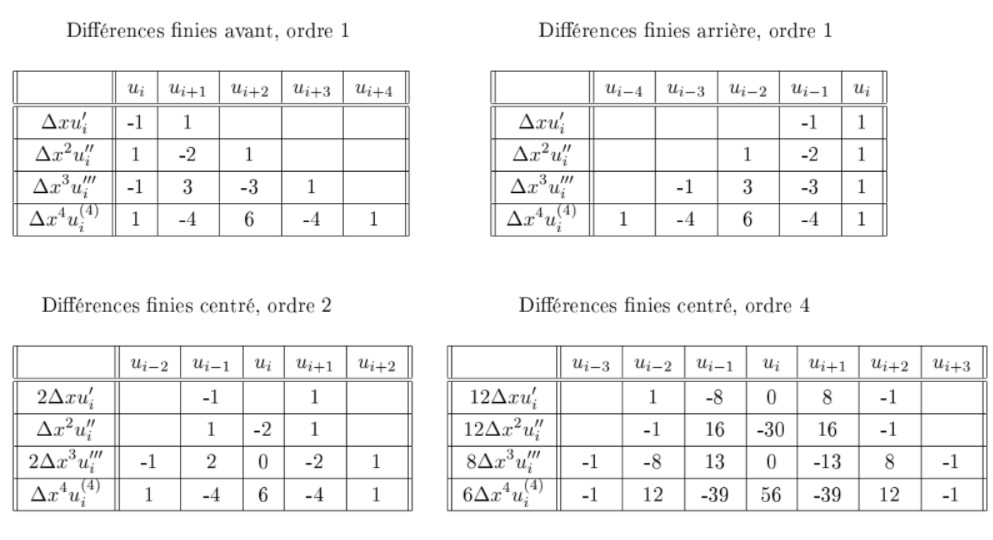
\includegraphics[width=1\textwidth]{./annex1}~\\[1cm]

\section{Solutions pour la partie comparaison}
\begin{figure}[H]
\begin{minipage}[b]{.46\linewidth}
\centering\epsfig{figure=exact.png,width=\linewidth}
\caption{Solution exacte
    \label{fig1}
    }
\end{minipage} \hfill
\begin{minipage}[b]{.46\linewidth}
\centering\epsfig{figure=explicite.png,width=\linewidth}
\caption{Euler explicite\label{fig2}}
\end{minipage}
\end{figure}

\begin{figure}[H]
\begin{minipage}[b]{.46\linewidth}
\centering\epsfig{figure=implicite.png,width=\linewidth}
\caption{Euler implicite\label{fig1}}
\end{minipage} \hfill
\begin{minipage}[b]{.46\linewidth}
\centering\epsfig{figure=RK.png,width=\linewidth}
\caption{Runge-Kutta \label{fig2}}
\end{minipage}
\end{figure}

\section{Algorithmes}
\subsection{Euler explicite}

\begin{enumerate}
    \item Initialisation des pas $\Delta x$ et $\Delta t$\\
    Initialisation des nombre de points du temps Nt et du nombre de points de l'espace Nx
    
    \item Calculs des conditions initiales $u^0_i$ et de $u^1_i$
    
    \item Calcul de la matrice trigonale A
    
    \item Tant que n<Nt faire:
        \begin{itemize}
        \item Calculs de $U^{n+1}_i$ : $U^{n+1}_i = A.U^{n}_i - U^{n-1}_i + C_i$\\
        \end{itemize}
    
\end{enumerate}

\subsection{Euler implicite}
\begin{enumerate}
    \item Initialisation des pas $\Delta x$ et $\Delta t$\\
    Initialisation des nombre de points du temps Nt et du nombre de points de l'espace Nx
    
    \item Calculs des conditions initiales $u^0_i$ et de $u^1_i$
    
    \item Calcul de la matrice trigonale A et de son inverse $A^{-1}$
    
    \item Tant que n<Nt faire:\\
        \begin{itemize}
            \item Calcul de $U^{n+1}_i$: $U^{n+1}_i = A^{-1}(U^{n}_i - \frac{1}{2}.U^{n-1}_i)$
        \end{itemize}
    
\end{enumerate}

\subsection{Runge-Kutta}
Algorithme utilisé dans le code python:
\begin{enumerate}
    \item Initialisation des pas $\Delta x$ et $\Delta t$\\
    Initialisation des nombre de points du temps Nt et du nombre de points de l'espace Nx
    
    \item Calculs des conditions initiales $u^0_{i}$ et de $(\frac{\partial u^n_{i}}{\partial t})^0_{i}$
    
    \item Tant que n<Nt faire:\\
     Tant que i<Nx faire:
        \begin{itemize}
            \item Calcul de $((k_0)_{i})$
            \item Calcul de $((l_0)_{i})$
            \item Calcul de $((k_1){i})$
            \item Calcul de $((l_1)_{i})$
            \item ...
            \item Calculs de $u^{n+1}_{i}$ et $(\frac{\partial u^n_{i}}{\partial t})^n_{i}$
        \end{itemize}
    
\end{enumerate}

\section{Lien Github}
Lien vers le répertoire Github contenant les différents codes python utilisés au cours du projet:\\
\url{https://github.com/Rudiio/Projet-Musique.git}

\section{Tests complémentaires pour la méthode de Runge-Kutta}
\begin{figure}[H]
\begin{minipage}[b]{.46\linewidth}
\centering\epsfig{figure=55.png,width=7cm}
\caption{
        $\Delta x= 5^{-2}m $\\
        $\Delta t= 10^{-7}s$\\
        $\lambda = 6.8.10^{-4}$
    \label{fig1}
    }
\end{minipage} \hfill
\begin{minipage}[b]{.46\linewidth}
\centering\epsfig{figure=44.png,width=7cm}
\caption{$\Delta x= 5^{-3}m $\\ 
        $\Delta t= 10^{-6}s$\\
        $\lambda = 0.068$
        \label{fig2}}
\end{minipage}
\end{figure}

\begin{figure}[H]
\begin{minipage}[b]{.46\linewidth}
\centering\epsfig{figure=9_stab.png,width=7cm}
\caption{$\Delta x= 5^{-4}m $\\ 
        $\Delta t= 1.47.10^{-6}s$\\
        $\lambda = 1$
        \label{fig1}
        }
\end{minipage} \hfill
\begin{minipage}[b]{.46\linewidth}
\centering\epsfig{figure=10.png,width=\linewidth}
\caption{$\Delta x= 3^{-3} m $\\ 
        $\Delta t= 10^{-6}s  $\\
        $\lambda = 0.113$
        \label{fig2}}
\end{minipage}
\end{figure}




%récupérer les citation avec "/footnotemark"
\nocite{*}

%choix du style de la biblio
\bibliographystyle{plain}
%inclusion de la biblio
\bibliography{Bibliographie.bib}
%voir wiki pour plus d'information sur la syntaxe des entrées d'une bibliographie

\end{document}